\documentclass[10pt,twoside]{book}
\usepackage{beamerarticle}
\usepackage{CJKutf8,CJKnumb}
\usepackage{amsmath,amssymb,amsthm,amscd}
\usepackage{wasysym}
\usepackage{gensymb}
\usepackage{titlesec}
\usepackage[paperwidth=185mm,paperheight=260mm,text={148mm,210mm},
			left=21mm,vmarginratio=1:1]{geometry}
\usepackage{enumitem}
\usepackage{tikz}
\usepackage{circuitikz}
%\usepackage{asymptote}
\usepackage[utf8]{inputenc}
\usepackage[unicode={true}]{hyperref}
\usepackage{manfnt}
\usepackage{array}
\usepackage{longtable}
\usepackage{multirow}
\usepackage{supertabular}
\usepackage{lscape}
\setjobnamebeamerversion{PLC.beamer}
\usetikzlibrary{positioning,calc}
\usetikzlibrary{shapes,snakes}
\tikzset{
>=stealth,
nonterminal/.style={rectangle,minimum size=6mm,draw=black,font=\ttfamily},
circleterminal/.style={circle,minimum size=1mm,draw=black}
}
\begin{document}
\titleformat{\chapter}[hang]{\centering\huge\bfseries}{\chaptername}{1em}{}
\setlength{\floatsep}{5pt plus 2pt minus 2pt}
\setlength{\abovecaptionskip}{2pt plus 1pt minus 1pt}
\setlength{\belowcaptionskip}{2pt plus 1pt minus 2pt}
\setenumerate[1]{itemsep=0pt,partopsep=0pt,parsep=\parskip,topsep=5pt}
\setitemize[1]{itemsep=0pt,partopsep=0pt,parsep=\parskip,topsep=5pt}
\setdescription{itemsep=0pt,partopsep=0pt,parsep=\parskip,topsep=5pt}
\begin{CJK}{UTF8}{song}
\title{\huge 《PLC技术》授课教案}
\author{\large 任\ 课\ 教\ 师:\underline{金波\qquad\qquad\qquad\quad}\\ 授\ 课\ 班\ 级:\underline{12电气控制及自动化}\\ 课程总学时:\underline{72\qquad\qquad\qquad\qquad}\\ 课\ 改\ 类\ 型:\underline{项目化课程\qquad\qquad}}
\date{二零一四年三月}
\maketitle
\chapter{平面图样绘制}
{\bfseries 知识目标}
\begin{itemize}
\item 了解国家制图标准和电气 AutoCAD 制图规范
\item 掌握平面图样的绘制步骤和方法
\item 掌握用 AutoCAD 绘制平面图样的基本步骤和方法
\item 掌握 AutoCAD 基本的绘图命令
\end{itemize}

{\bfseries 技能目标}
\begin{itemize}
\item 具备平面样抄绘能力
\item 具备使用AutoCAD绘制中等复杂程度的图样的能力
\item 具备阅读和分析平面图样的能力
\end{itemize}

{\bfseries 本章导引}

图\ref{fig:shangmu1}所示图纸即为图样,是根据投影法,并按照国家或国际标准的规定绘制的,用于工程施工或产品制造等用途的图。标准则是为了在一定范围内获得最佳秩序,而对活动或其结果规定共同的和重复使用的规则、导则或特性的文件。本章旨在通过讲解图\ref{fig:shangmu1}所示项目,使学生在完成项目的同时,了解和掌握国家制图标准中图幅、比例、线型、文字、标注等相关知识,以及通过AutoCAD进行图样绘制的步骤、方法、技巧和规范,并能运用所学的技巧和知识解决绘图过程中的实际问题,具备遵照国家制图标准和规范抄绘图样的能力。
\noindent
\begin{landscape}
\begin{figure}[htbp]
\centering
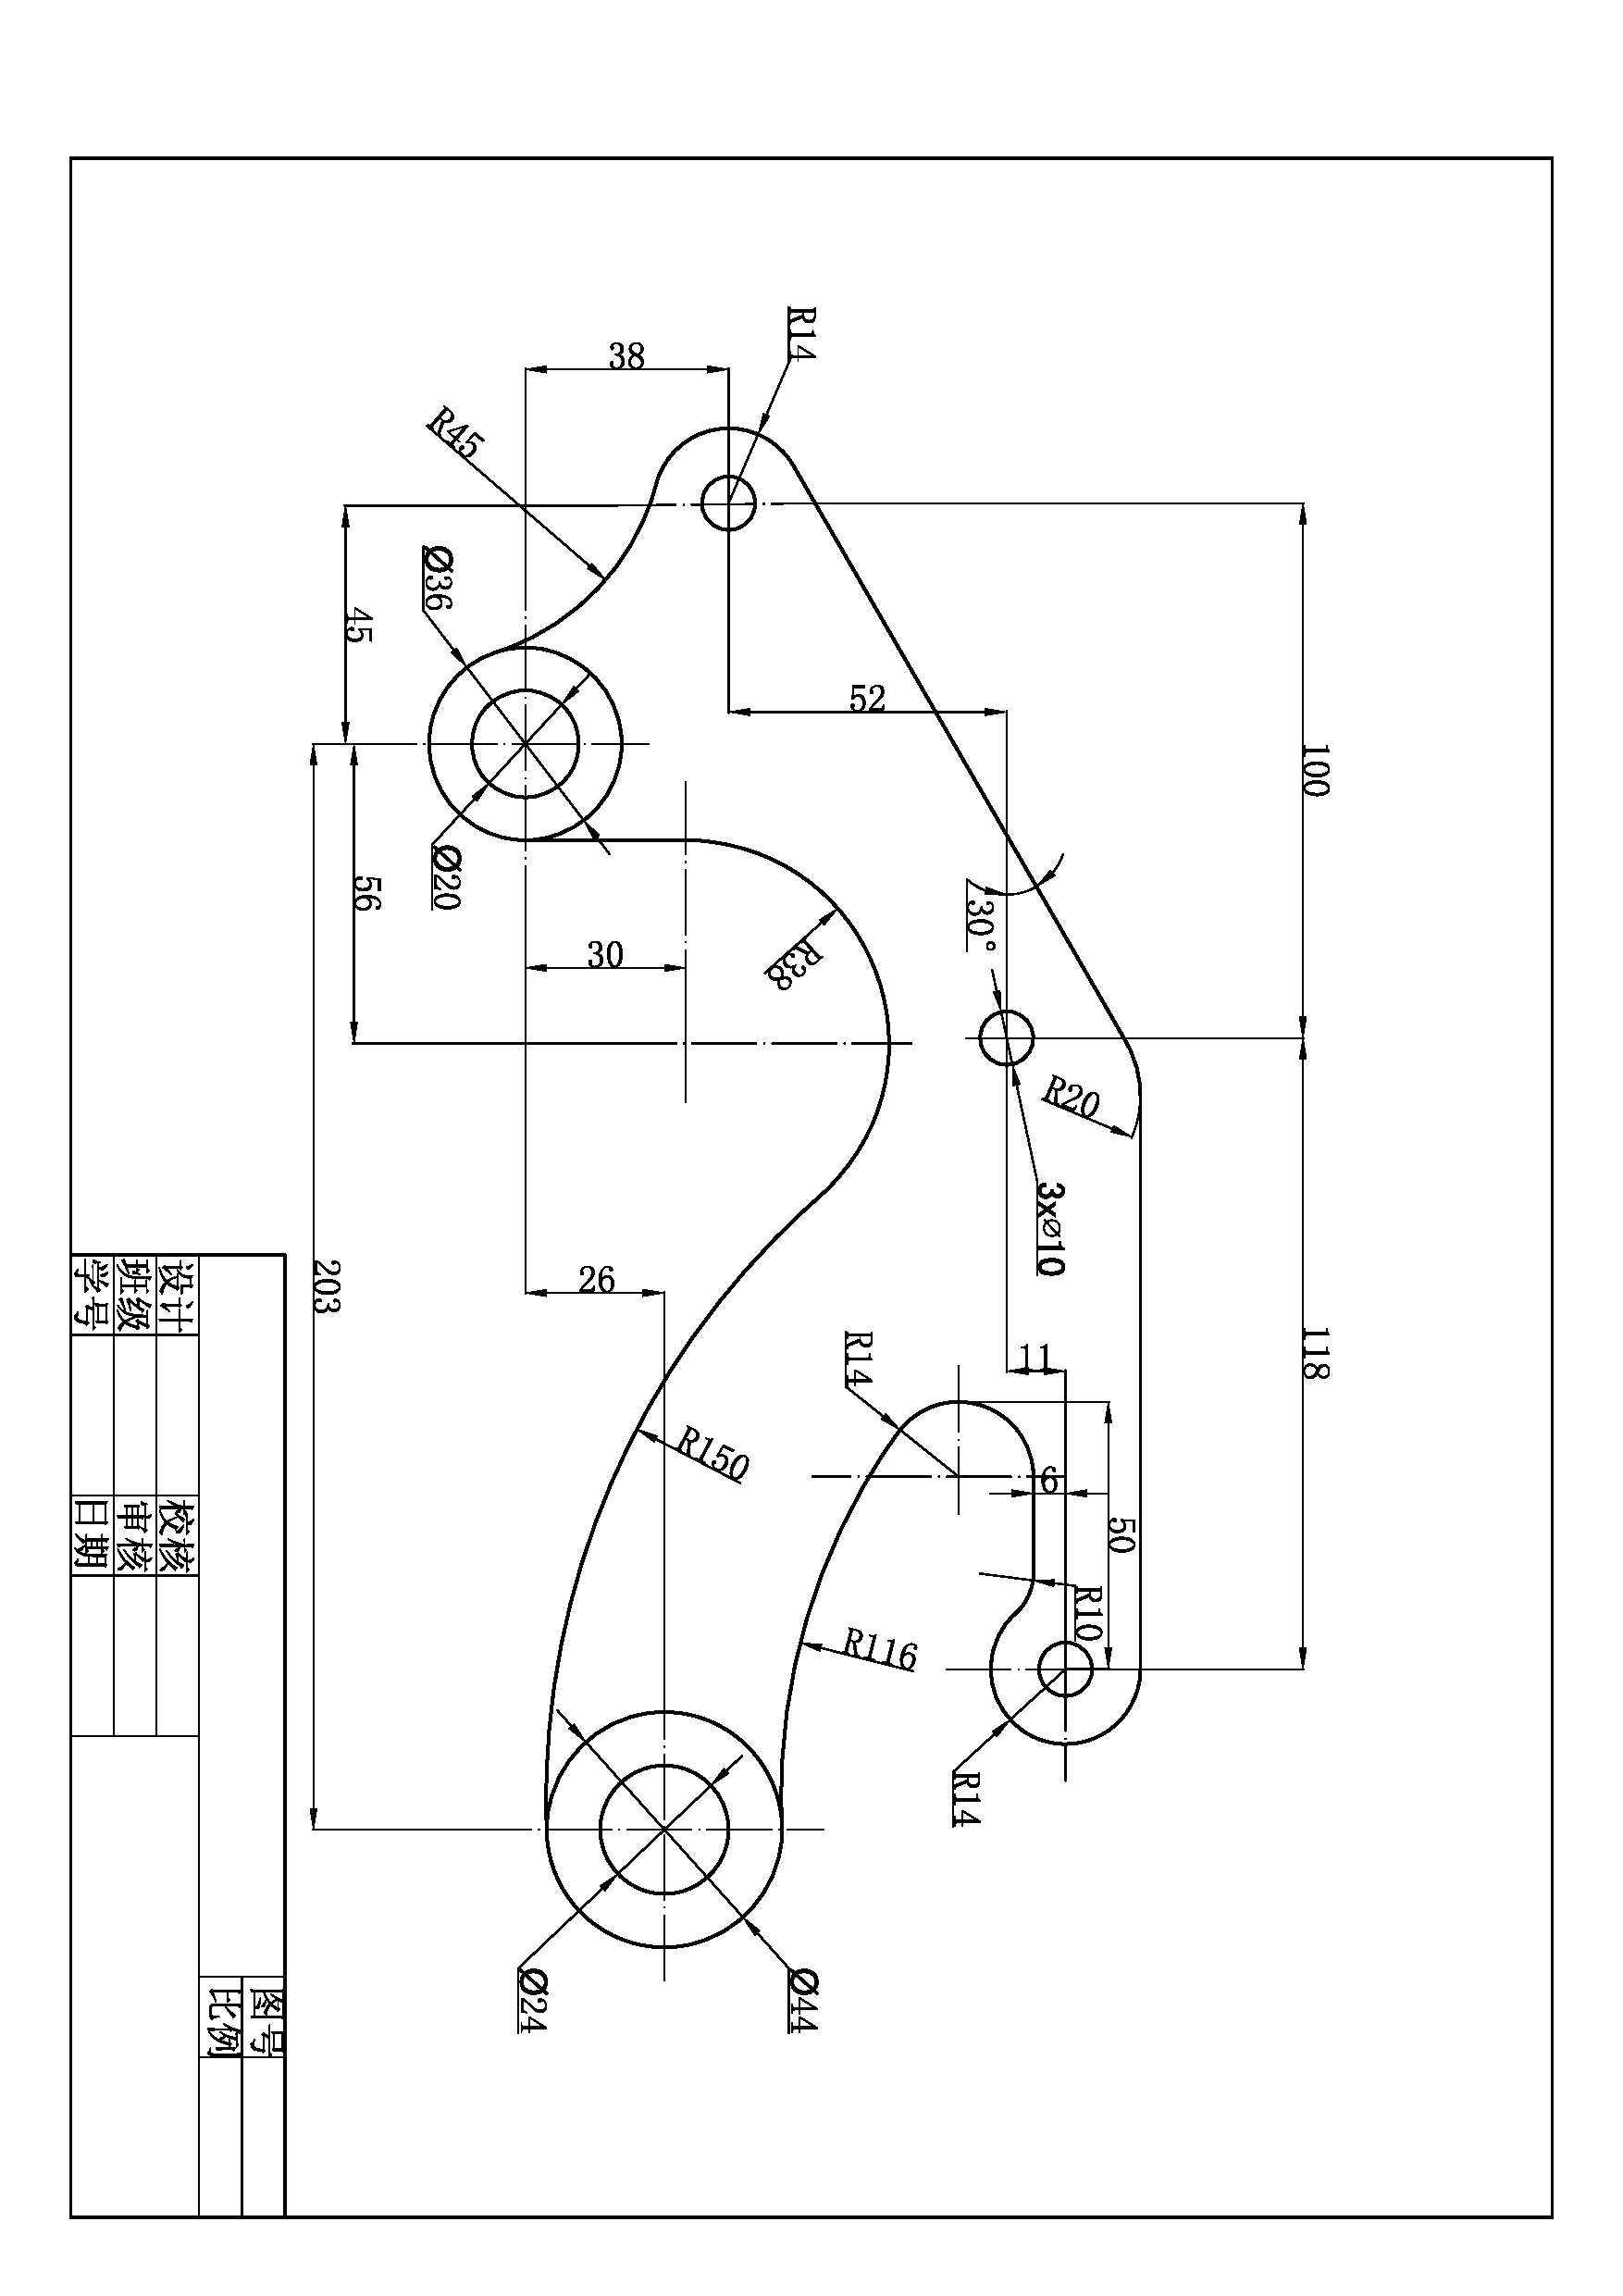
\includegraphics[scale=0.45,angle=90]{shu1.pdf}
\caption{项目一示例}\label{fig:shangmu1}
\end{figure}
\end{landscape}
\indent
%\newpage

\section{平面几何图(一)}\label{sec:gongzhi}

{\bfseries 知识目标}
\begin{itemize}
\item 掌握绝对坐标、相对坐标和极轴坐标的概念
\item 掌握limits命令的使用方法
\item 掌握point、line命令的使用方法
\item 了解国家制图标准中图幅的标准及与limits命令之间的关系
\end{itemize}

{\bfseries 技能目标}
\begin{itemize}
\item 能够完成工字图样的绘制
\end{itemize}

本任务以绘制图\ref{fig:shangmu1-1}所示的工字图样为目标,主要是为了帮助读者掌握Auto\-CAD 图形绘制过程中最重要的概念---坐标。坐标是AutoCAD精确绘的基础,对图形对象的精确定位起至关重要的作用。通过完成该任务来理解AutoCAD中图形的关键点的坐标描述方法,以及各种坐标表述方式的应用情景。其次是为了让读者掌握line命令的基本用法。
\enlargethispage{10pt}
\noindent
\begin{figure}[htbp]
\centering
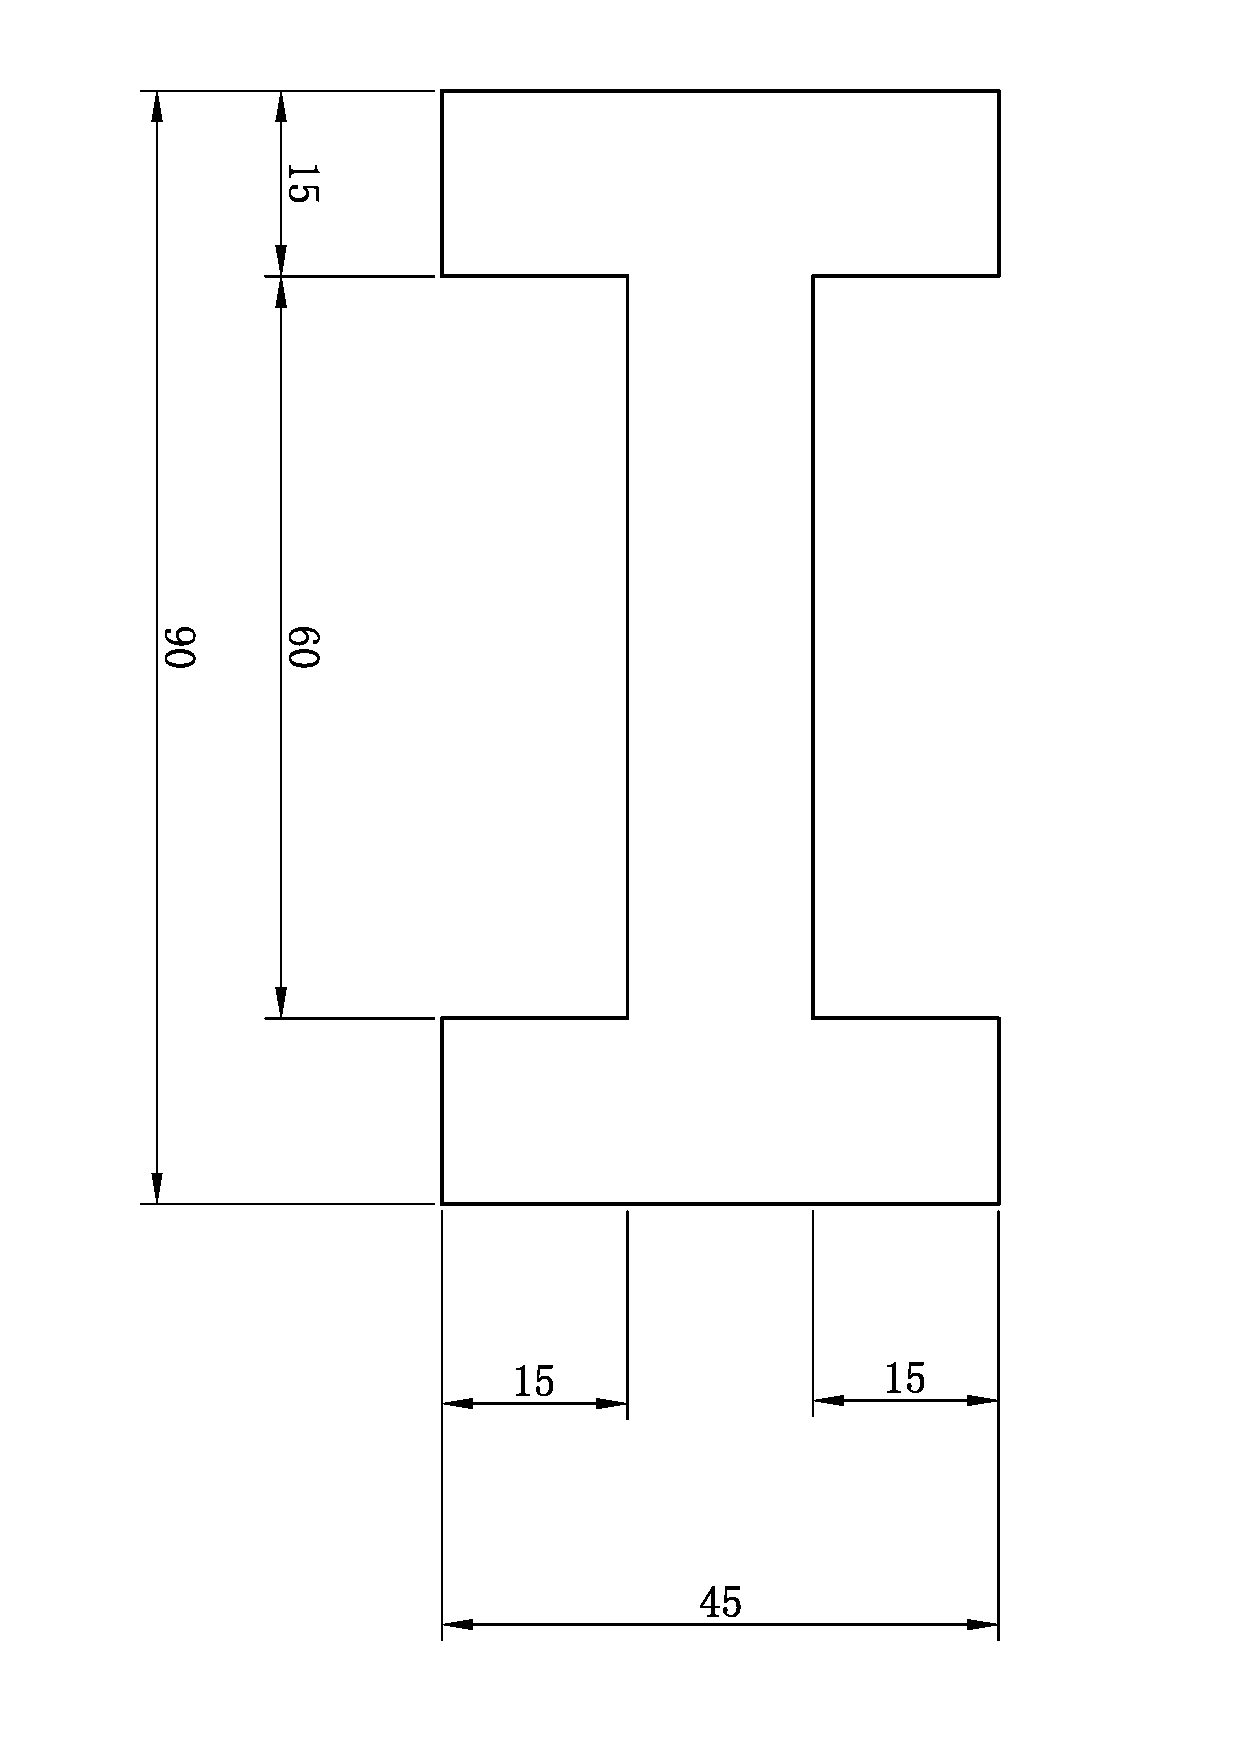
\includegraphics[scale=0.4,angle=90]{gongzi.pdf}
\caption{工字图样}\label{fig:shangmu1-1}
\end{figure}
\indent

\subsection{绘制图样}
\subsubsection{设置图形界限LIMITS}
AutoCAD中的绘图区域是无限大的,可以在绘图区的任何地方绘图。为一方便打印,一般需要设置一个绘图区域用来限制绘图的区域,不至于将图形绘制来区域之外。要实现此功能,用户使用“图形界限”命令进行设置。

在命令提示区输入limits 以执行“图形界限”命令。
\noindent
命令:  LIMITS\\
重新设置模型空间界限:\\
指定左下角点或 [开(ON)/关(OFF)] $<$0.0000,0.0000$>$:\\
指定右上角点 $<$420.0000,297.0000$>$: 297,210\\
\indent
LIMITS命令中【开(ON)】表示打开界限检查,此时不能够在图形界限以外输入点来创建图形对象。【关(OFF)】表示关闭界限检查,此时能够在图形界限以外输入图形对象。

\subsubsection{图形缩放显示ZOOM}
由于图\ref{fig:shangmu1-1}的尺寸比较小,为了便于观察绘图结果,我们需要先使用ZOOM命令先将图形显示区域缩放到图形界限范围。

\noindent
命令: ZOOM\\
指定窗口的角点,输入比例因子 (nX 或 nXP),或者
[全部(A)/中心(C)/动态(D)/范围(E)/上一个(P)/比例(S)/窗口(W)/对象(O)] $<$实时$>$: a
\indent

ZOOM命令中各个选项的含义如下:
\begin{itemize}
\item 全部(A):在平面图形中,缩放到整个图形界限
\item 中心(C):缩放显示由中心点和缩放比例(或高度)所定义的窗口
\item 动态(D):执行此选项,会出现一个视图框,通过调整视图框的大小,调整显示图形的大小
\item 范围(E):最大限度的显示所有图形
\item 上一个(P):回到上一次缩放
\item 比例(s):按输入比例值进行缩放
\item 窗口(W):最大限度地显示框选的图形
\item 对象(O):最大限度地显示选择的对象
\end{itemize}
\subsubsection{绘制图形}
绘制图\ref{fig:shangmu1-1}需要使用AutoCAD中的line命令。

\noindent
命令: line 指定第一点: 0,0\\
指定下一点或 [放弃(U)]: @0,45\\
指定下一点或 [放弃(U)]: @15,0\\
指定下一点或 [闭合(C)/放弃(U)]: @-15$<$90\\
指定下一点或 [闭合(C)/放弃(U)]: @60$<$0\\
指定下一点或 [闭合(C)/放弃(U)]: @15$<$90\\
指定下一点或 [闭合(C)/放弃(U)]: @15$<$0\\
指定下一点或 [闭合(C)/放弃(U)]: @45$<$-90\\
指定下一点或 [闭合(C)/放弃(U)]: @15$<$180\\
指定下一点或 [闭合(C)/放弃(U)]: @15$<$90\\
指定下一点或 [闭合(C)/放弃(U)]: @-60$<$0\\
指定下一点或 [闭合(C)/放弃(U)]: @-15$<$90\\
指定下一点或 [闭合(C)/放弃(U)]: c

\indent
line命令中【放弃(U)】表示删除直线序列中最近绘制的线段。【闭合(C)】表示当以第一条线段的起点和最后一线段的端点,形成一个闭合的线段环。注意到上面的提示序列,只有线段数大于等两条时该选项才可以使用。

\zhishi{坐标理论}
坐标是精确定位AutoCAD对象的基础,在\ref{sec:gongzhi}中使用了$(x,y)$、$(@x,y)$ 和 $(@$距离$<$角度$)$三种形式来表示式字图形的各个牲点位置。此种形式即为Auto\-CAD 的坐标表示方式。
\subsection{卡笛尔坐标系}
卡笛尔坐标系即为直角坐标系,是用通过原点$O(0,0)$的两个相互垂直的坐标轴$X$和$Y$来表示绘图区域。图中的每一个点均表示为$(x,y)$的形式,如图\ref{fig:zuobiao1}所示。
\begin{figure}[htbp]
\centering
\begin{floatrow}
\ffigbox{\caption{坐标表示}\label{fig:zuobiao1}}{
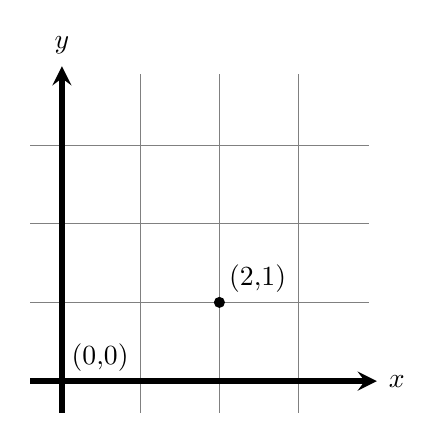
\begin{tikzpicture}
\draw[help lines,step=1cm,very thin](-0.4cm,-0.4cm)grid(3.9cm,3.9cm);
\draw[->,line width=0.7mm](-0.4cm,0)--(4cm,0)node[right]{$x$};
\draw[->,line width=0.7mm](0,-0.4cm)--(0,4cm)node[above]{$y$};
\draw (0,0)node[above right]{(0,0)};
\fill (2cm,1cm)node[above right]{(2,1)}circle(2pt);
\end{tikzpicture}}
\ffigbox{\caption{极坐标表示}\label{fig:jizuobiao1}}{
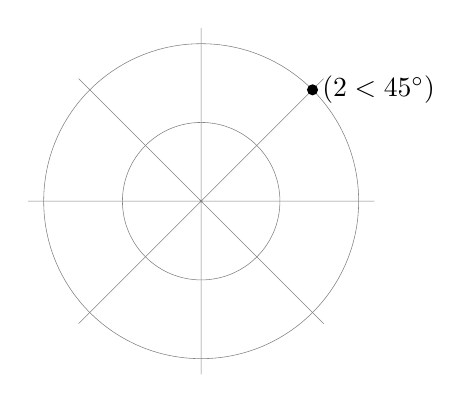
\begin{tikzpicture}
\draw[help lines,very thin](-2.2cm,0)--(2.2cm,0)(0,-2.2cm)--(0,2.2cm)(45:2.2cm)--(225:2.2cm)(135:2.2cm)--(-45:2.2cm);
\draw[help lines,very thin](0,0)circle(1cm)circle(2cm);
\fill (45:2cm)node[right]{$(2<45\degree)$}circle(2pt);
\end{tikzpicture}
}
\end{floatrow}
\end{figure}
\subsection{极坐标系}
极坐标系是一个二维坐标系统,它用一段相对于中心点的距离和一个夹角来表示坐标区域中的点,其坐形式为$(\rho,\theta)$,如图\ref{fig:jizuobiao1}所示。其中$\rho$表示距离,永远取正值,$\theta$表示角度,取值范围为$0-360\degree$。
\subsection{绝坐标和相对坐标}
绝对坐标是以当前坐标原点为基点进行参照所获得的坐标值。如$(3,5)$,$(4<45\degree)$。

相对坐标是以前面输入的坐标点为参照所获得的坐标值,表示方法是在坐标值前面加一个“@”符号。例如,相对直角坐标表示为$(@5,4)$,相对极坐标表示为$(@5<35)$。

例如,绘制一条两个端点分别为$(3,5)$和$(6,9)$的直线。调用line命令:

\noindent
命令: line 指定第一点: 3,5\\
指定下一点或 [放弃(U)]:\\
用绝对坐标方式输入,$(6,9)$就可以绘出直线。\\
用相对坐标方式输入,可知$(6,9)$相对于$(3,5)$的$X$轴增量为3,$Y$轴增量为4,故输入相对坐标$(@3,4)$也可以绘出直线。

\indent
但是,从AutoCAD的实际绘图过程来看,多种坐标输入方式配合使用会使整个绘图过程更加灵活和方便,再配合目标捕捉和夹点编辑等方式,则使绘图更精确、更快捷。
\zhishi{图纸幅面及格式}
\subsection{图纸幅面}
“图形界限”中我们所设置的297$\times $210的尺寸就是国家标准中的A4图纸幅面。国家标准《技术制图》中规定幅面的尺寸是为了方便绘制、使用和保管图样。因此,在绘制图样时,应优先采用表\ref{tab:tufubiao1}中规定的尺寸,必要时允许先用规定的加长幅面,加长幅面的尺寸由基本幅面短边的成整数倍增加后得出,如图\ref{fig:tufujiachang}所示。其中粗实细部分为基本幅面。加长后幅面记作:基本幅面代号$\times $倍数。如$A3\times 3$,表示按A3图幅短边加长为297mm的3倍,即加长后图纸尺寸为$420mm\times 891mm$。
%\suppressfloats[t]
\begin{table}[htbp]
\caption{图纸幅面及周边尺寸}\label{tab:tufubiao1}
\begin{tabular}{*{6}{c|}c}
\hline
\multicolumn{2}{c|}{幅面代号}&A0&A1&A2&A3&A4\\ \hline
\multicolumn{2}{c|}{尺寸 $B\times L$}&$841\times 1189$&$594\times 841$&$420\times 594$&$297\times 420$&$210\times 297$\\ \hline
\multirow{3}*{图框}&a&\multicolumn{5}{|c}{25}\\ \cline{2-7}
&c&\multicolumn{3}{|c}{10}&\multicolumn{2}{|c}{5}\\ \cline{2-7}
&e&\multicolumn{2}{|c}{20}&\multicolumn{3}{|c}{10}\\
\hline
\end{tabular}
\end{table}

\begin{figure}[htbp]
\centering
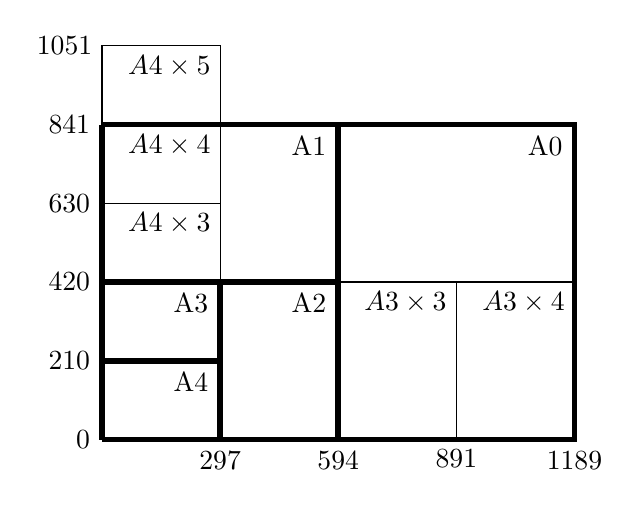
\begin{tikzpicture}
\draw[line width=0.7mm] (0,0)node[left]{0}--(0,1cm)node[left]{210}--(0,2cm)node[left]{420}--(0,3cm)node[left]{630}--(0,4cm)node[left]{841};
\draw(0,4cm)--(0,5cm)node[left]{1051}--(1.5cm,5cm)node[below left]{$A4\times 5$}--(1.5cm,2cm);
\draw[line width=0.7mm](0,1cm)--(1.5cm,1cm)node[below left]{A4}(0,2cm)--(1.5cm,2cm)node[below left]{A3}--(1.5cm,0)node[below]{297};
\draw(0,3cm)--(1.5cm,3cm)node[below left]{$A4\times 3$};
\draw[line width=0.7mm](0,4cm)--(3cm,4cm)node[below left]{A1}--(3cm,0)node[below]{594}(1.5cm,2cm)--(3cm,2cm)node[below left]{A2};
\draw[line width=0.7mm](3cm,4cm)--(6cm,4cm)node[below left]{A0}--(6cm,0)node[below]{1189}--(0,0);
\draw(3cm,2cm)--(4.5cm,2cm)node[below left]{$A3\times 3$}--(6cm,2cm)node[below left]{$A3\times 4$}(4.5cm,2cm)--(4.5cm,0)node[below]{891};
\draw(1.5cm,4cm)node[below left]{$A4\times 4$};
\end{tikzpicture}
\caption{图纸幅面及加长边} \label{fig:tufujiachang}
\end{figure}

从表\ref{tab:tufubiao1}中可以看出幅面之间的关系为:将A0图纸的长边对折后得到两张A1图纸,将A1图纸的长边对折后得到两纸A2图纸,以此类推。

\subsection{标题栏}
每张图样上必须画出标题栏,标题栏位于图样的右下角,与看图的方向一致。

标题栏分为更必区、签字区、名称及代号区和其他区,如图\ref{fig:biaotilan}所示。
\tikzset{
>=latex,
center lines/.style={dash pattern=on 20pt off 3pt on 2pt off 3pt},
importance lines/.style={line width=1pt}
}
\noindent
\begin{figure}[htbp]
\begin{tikzpicture}[scale=0.65]
\draw[line width=0.7mm](0,0)rectangle(180mm,56mm);
\draw(0,7mm)--(12mm,7mm)--(40mm,7mm)--++(40mm,0);
\draw(6mm,3.5mm)node{\tiny 工艺};
\draw(46mm,3.5mm)node{\tiny 批准};
\draw(0,14mm)--++(80mm,0);
\draw(6mm,10.5mm)node{\tiny 审核};
\draw(0,21mm)--++(12mm,0)--++(12mm,0)--++(16mm,0)--++(12mm,0)--++(12mm,0)--++(16mm,0);
\draw(6mm,24.5mm)node{\tiny设计};
\draw(18mm,24.5mm)node{\tiny(签名)};
\draw(32mm,24.5mm)node{\tiny(年月日)};
\draw(46mm,24.5mm)node{\tiny标准化};
\draw(58mm,24.5mm)node{\tiny签名};
\draw(72mm,24.5mm)node{\tiny(年月日)};
\draw(12mm,0)--++(0,28mm)(24mm,0)--++(0,28mm)(40mm,0)--++(0,28mm)(52mm,0)--++(0,28mm)(64mm,0)--++(0,28mm)(80mm,0)--++(0,28mm);
\draw(0,28mm)--++(10mm,0)--++(10mm,0)--++(16mm,0)--++(16mm,0)--++(12mm,0)--++(16mm,0);
\draw(5mm,31.5mm)node{\tiny 标记};
\draw(15mm,31.5mm)node{\tiny 处数};
\draw(28mm,31.5mm)node{\tiny 分区};
\draw(44mm,31.5mm)node{\tiny 更改文件号};
\draw(56mm,31.5mm)node{\tiny 签名};
\draw(72mm,31.5mm)node{\tiny 年月日};
\draw(0,35mm)--++(80mm,0)(0,42mm)--++(80mm,0)(0,49mm)--++(80mm,0);
\draw(10mm,28mm)--++(0,28mm)(20mm,28mm)--++(0,28mm)(36mm,28mm)--++(0,28mm)(52mm,28mm)--++(0,28mm)(64mm,28mm)--++(0,28mm)(80mm,28mm)--++(0,28mm);
\draw(80mm,9mm)--++(50mm,0);
\draw(105mm,4.5mm)node{\tiny 共\quad张\quad第\quad张};
\draw(80mm,18mm)--++(26mm,0)--++(12mm,0)--++(12mm,0);
\draw(93mm,23mm)node{\tiny 阶段标记};
\draw(112mm,23mm)node{\tiny 重量};
\draw(124mm,23mm)node{\tiny 比例};
\draw(86.5mm,9mm)--++(0,9mm)(93mm,9mm)--++(0,9mm)(99.5mm,9mm)--++(0,9mm)(106mm,9mm)--++(0,18mm)(118mm,9mm)--++(0,18mm);
\draw(80mm,28mm)--++(50mm,0);
\draw(130mm,0)--++(0,56mm);
\draw(130mm,18mm)--++(50mm,0)(130mm,38mm)--++(50mm,0);
\draw (155mm,9mm)node{\tiny(图样代号)};
\draw(155mm,28mm)node{\tiny(图样名称)};
\draw(155mm,48mm)node{\tiny(单位名称)};
\draw(105mm,48mm)node{\tiny(材料标记)};
\draw[<->](99.5mm,12mm)--(106mm,12mm)node[midway,above]{\tiny 6.5};
\draw(-14mm,0)--(0,0)(-7mm,7mm)--(0,7mm)(-14mm,56mm)--(0,56mm);
\draw[<->](-5mm,0)--(-5mm,7mm)node[midway,above,rotate=90]{\tiny 7};
\draw[<->](-13mm,0)--(-13mm,56mm)node[midway,above,rotate=90]{\tiny $8\times 7(56)$};
\draw(130mm,9mm)--++(9mm,0)(130mm,28mm)--++(9mm,0);
\draw[<->](137mm,0)--++(0,9mm)node[midway,above,rotate=90]{\tiny 9};
\draw[<->](137mm,9mm)--++(0,9mm)node[midway,above,rotate=90]{\tiny 9};
\draw[<->](137mm,18mm)--++(0,10mm)node[midway,above,rotate=90]{\tiny 10};
\draw(180mm,0)--++(9mm,0)(180mm,18mm)--++(9mm,0)(180mm,38mm)--++(9mm,0);
\draw[<->](187mm,0)--++(0,18mm)node[midway,above,rotate=90]{\tiny 18};
\draw[<->](187mm,18mm)--++(0,20mm)node[midway,above,rotate=90]{\tiny 20};
\draw(0,-9mm)--++(0,9mm)(12mm,-9mm)--++(0,9mm)(24mm,-9mm)--++(0,9mm)(40mm,-9mm)--++(0,9mm)(52mm,-9mm)--++(0,9mm)(64mm,-9mm)--++(0,9mm)(80mm,-9mm)--++(0,9mm)(130mm,-9mm)--++(0,9mm);
\draw[<->](0,-7mm)--++(12mm,0)node[midway,above]{\tiny 12};
\draw[<->](12mm,-7mm)--++(12mm,0)node[midway,above]{\tiny 12};
\draw[<->](24mm,-7mm)--++(16mm,0)node[midway,above]{\tiny 16};
\draw[<->](40mm,-7mm)--++(12mm,0)node[midway,above]{\tiny 12};
\draw[<->](52mm,-7mm)--++(12mm,0)node[midway,above]{\tiny 12};
\draw[<->](64mm,-7mm)--++(16mm,0)node[midway,above]{\tiny 16};
\draw[<->](80mm,-7mm)--++(50mm,0)node[midway,above]{\tiny 50};
\draw(0,-18mm)--(0,0)(180mm,-18mm)--(180mm,0);
\draw[<->](0,-16mm)--(180mm,-16mm)node[midway,above]{\tiny 180};
\draw(0,56mm)--++(0,7mm)(10mm,56mm)--++(0,7mm)(20mm,56mm)--++(0,7mm)(36mm,56mm)--++(0,7mm)(52mm,56mm)--++(0,7mm)(64mm,56mm)--++(0,7mm)(80mm,56mm)--++(0,7mm);
\draw[<->](0,61mm)--++(10mm,0)node[midway,above]{\tiny 10};
\draw[<->](10mm,61mm)--++(10mm,0)node[midway,above]{\tiny 10};
\draw[<->](20mm,61mm)--++(16mm,0)node[midway,above]{\tiny 16};
\draw[<->](36mm,61mm)--++(16mm,0)node[midway,above]{\tiny 16};
\draw[<->](52mm,61mm)--++(12mm,0)node[midway,above]{\tiny 12};
\draw[<->](64mm,61mm)--++(16mm,0)node[midway,above]{\tiny 16};
\draw(106mm,28mm)--++(0,7mm)(118mm,28mm)--++(0,7mm);
\draw[<->](80mm,33mm)--++(26mm,0)node[midway,above]{\tiny $4\times 6.5(26)$};
\draw[<->](106mm,33mm)--++(12mm,0)node[midway,above]{\tiny 12};
\draw[<->](118mm,33mm)--++(12mm,0)node[midway,above]{\tiny 12};
\end{tikzpicture}
\caption{标题栏格式及尺寸}\label{fig:biaotilan}
\end{figure}
\indent

\subsection{图框格式}
图框格式分为留装订边和不留装订边两种,其装订边尺寸如表\ref{tab:tufubiao1}所示。图\ref{fig:zhuangding}所示为采用A4幅面竖装和A3幅面横装时,留装订边和不留装订边的图框格式。
\noindent
\tikzset{
>=latex,
center lines/.style={dash pattern=on 20pt off 3pt on 2pt off 3pt},
importance lines/.style={line width=1pt}
}
\begin{figure}[htbp]
\centering
\subfloat[留装订边格式]{
\begin{tikzpicture}
\draw(0,0)rectangle(4cm,5cm);
\draw[line width=0.7mm](0.5cm,0.25cm)rectangle(3.75cm,4.75cm)(1.5cm,0.25cm)--(1.5cm,1cm)--(3.75cm,1cm)node[midway,below]{标题栏};
\draw(-0.7cm,0)--(0,0)(-0.7cm,5cm)--(0cm,5cm);
\draw[<->](-0.5cm,0)--(-0.5cm,5cm)node[midway,above,rotate=90]{$L$};
\draw(0,-0.7cm)--(0,0)(4cm,-0.7cm)--(4cm,0);
\draw[<->](0,-0.5cm)--(4cm,-0.5cm)node[midway,above]{$B$};
\draw[->](1cm,-0.45cm)--(1cm,0);
\draw[->](1cm,0.65cm)--(1cm,0.25cm)node[midway,above,rotate=90]{$c$};
\draw(1cm,0)--(1cm,0.25cm);
\draw[->](-0.4cm,2cm)--(0,2cm);
\draw[->](0.9cm,2cm)--(0.5cm,2cm);
\draw(0,2cm)--(0.5cm,2cm)node[midway,above]{$a$};
\draw[->](2cm,5cm)--(2cm,4.35cm)--(2cm,4.75cm);
\draw[->](2cm,5.45cm)--(2cm,5cm)node[midway,above,rotate=90]{$c$};
\draw[->](4cm,2.5cm)--(3.3cm,2.5cm)--(3.75cm,2.5cm);
\draw[->](4.45cm,2.5cm)--(4cm,2.5cm)node[midway,above]{$c$};

\begin{scope}[xshift=5.5cm]
\draw(0,0)rectangle(7cm,5cm);
\draw[line width=0.7mm](0.5cm,0.25cm)rectangle(6.75cm,4.75cm)(4.5cm,0.25cm)--(4.5cm,1cm)--(6.75cm,1cm)node[midway,below]{标题栏};
\draw(-0.7cm,0)--(0,0)(-0.7cm,5cm)--(0cm,5cm);
\draw[<->](-0.5cm,0)--(-0.5cm,5cm)node[midway,above,rotate=90]{$B$};
\draw(0,-0.7cm)--(0,0)(7cm,-0.7cm)--(7cm,0);
\draw[<->](0,-0.5cm)--(7cm,-0.5cm)node[midway,above]{$L$};
\draw[->](3cm,-0.45cm)--(3cm,0);
\draw[->](3cm,0.65cm)--(3cm,0.25cm)node[midway,above,rotate=90]{$c$};
\draw(3cm,0)--(3cm,0.25cm);
\draw[->](-0.4cm,2cm)--(0,2cm);
\draw[->](0.9cm,2cm)--(0.5cm,2cm);
\draw(0,2cm)--(0.5cm,2cm)node[midway,above]{$a$};
\draw[->](3.5cm,5cm)--(3.5cm,4.35cm)--(3.5cm,4.75cm);
\draw[->](3.5cm,5.45cm)--(3.5cm,5cm)node[midway,above,rotate=90]{$c$};
\draw[->](7cm,2.5cm)--(6.3cm,2.5cm)--(6.75cm,2.5cm);
\draw[->](7.45cm,2.5cm)--(7cm,2.5cm)node[midway,above]{$c$};
\end{scope}
\end{tikzpicture}}

\subfloat[不留装订边格式]{
\begin{tikzpicture}
\draw(0,0)rectangle(4cm,5cm);
\draw[line width=0.7mm](0.25cm,0.25cm)rectangle(3.75cm,4.75cm)(1.5cm,0.25cm)--(1.5cm,1cm)--(3.75cm,1cm)node[midway,below]{标题栏};
\draw(-0.7cm,0)--(0,0)(-0.7cm,5cm)--(0cm,5cm);
\draw[<->](-0.5cm,0)--(-0.5cm,5cm)node[midway,above,rotate=90]{$L$};
\draw(0,-0.7cm)--(0,0)(4cm,-0.7cm)--(4cm,0);
\draw[<->](0,-0.5cm)--(4cm,-0.5cm)node[midway,above]{$B$};
\draw[->](1cm,-0.45cm)--(1cm,0);
\draw[->](1cm,0.65cm)--(1cm,0.25cm)node[midway,above,rotate=90]{$c$};
\draw(1cm,0)--(1cm,0.25cm);
\draw[->](-0.4cm,2cm)--(0,2cm);
\draw[->](0.65cm,2cm)--(0.25cm,2cm)node[midway,above]{$c$};
\draw(0,2cm)--(0.25cm,2cm);
\draw[->](2cm,5cm)--(2cm,4.35cm)--(2cm,4.75cm);
\draw[->](2cm,5.45cm)--(2cm,5cm)node[midway,above,rotate=90]{$c$};
\draw[->](4cm,2.5cm)--(3.3cm,2.5cm)--(3.75cm,2.5cm);
\draw[->](4.45cm,2.5cm)--(4cm,2.5cm)node[midway,above]{$c$};

\begin{scope}[xshift=5.5cm]
\draw(0,0)rectangle(7cm,5cm);
\draw[line width=0.7mm](0.25cm,0.25cm)rectangle(6.75cm,4.75cm)(4.5cm,0.25cm)--(4.5cm,1cm)--(6.75cm,1cm)node[midway,below]{标题栏};
\draw(-0.7cm,0)--(0,0)(-0.7cm,5cm)--(0cm,5cm);
\draw[<->](-0.5cm,0)--(-0.5cm,5cm)node[midway,above,rotate=90]{$B$};
\draw(0,-0.7cm)--(0,0)(7cm,-0.7cm)--(7cm,0);
\draw[<->](0,-0.5cm)--(7cm,-0.5cm)node[midway,above]{$L$};
\draw[->](3cm,-0.45cm)--(3cm,0);
\draw[->](3cm,0.65cm)--(3cm,0.25cm)node[midway,above,rotate=90]{$c$};
\draw(3cm,0)--(3cm,0.25cm);
\draw[->](-0.4cm,2cm)--(0,2cm);
\draw[->](0.65cm,2cm)--(0.25cm,2cm)node[midway,above]{$c$};
\draw(0,2cm)--(0.25cm,2cm);
\draw[->](3.5cm,5cm)--(3.5cm,4.35cm)--(3.5cm,4.75cm);
\draw[->](3.5cm,5.45cm)--(3.5cm,5cm)node[midway,above,rotate=90]{$c$};
\draw[->](7cm,2.5cm)--(6.3cm,2.5cm)--(6.75cm,2.5cm);
\draw[->](7.45cm,2.5cm)--(7cm,2.5cm)node[midway,above]{$c$};
\end{scope}
\end{tikzpicture}}
\caption{图框格式}\label{fig:zhuangding}
\end{figure}
\indent
\clearpage
\section{平面几何作图(二)}

{\bfseries 知识目标}
\begin{itemize}
\item 掌握layger命令和图层定义和使用方法
\item 掌握xline命令的使用方法
\item 掌握circle命令的使用方法
\item 掌握多边形命令的使用方法
\item 掌握图形阵列命令的使用方法
\end{itemize}

{\bfseries 技能目标}
\begin{itemize}
\item 能够完成简单图样的绘制
\item 具备用AutoCAD图层管理图线的能力
\end{itemize}

\noindent
\begin{figure}[htbp]
\centering
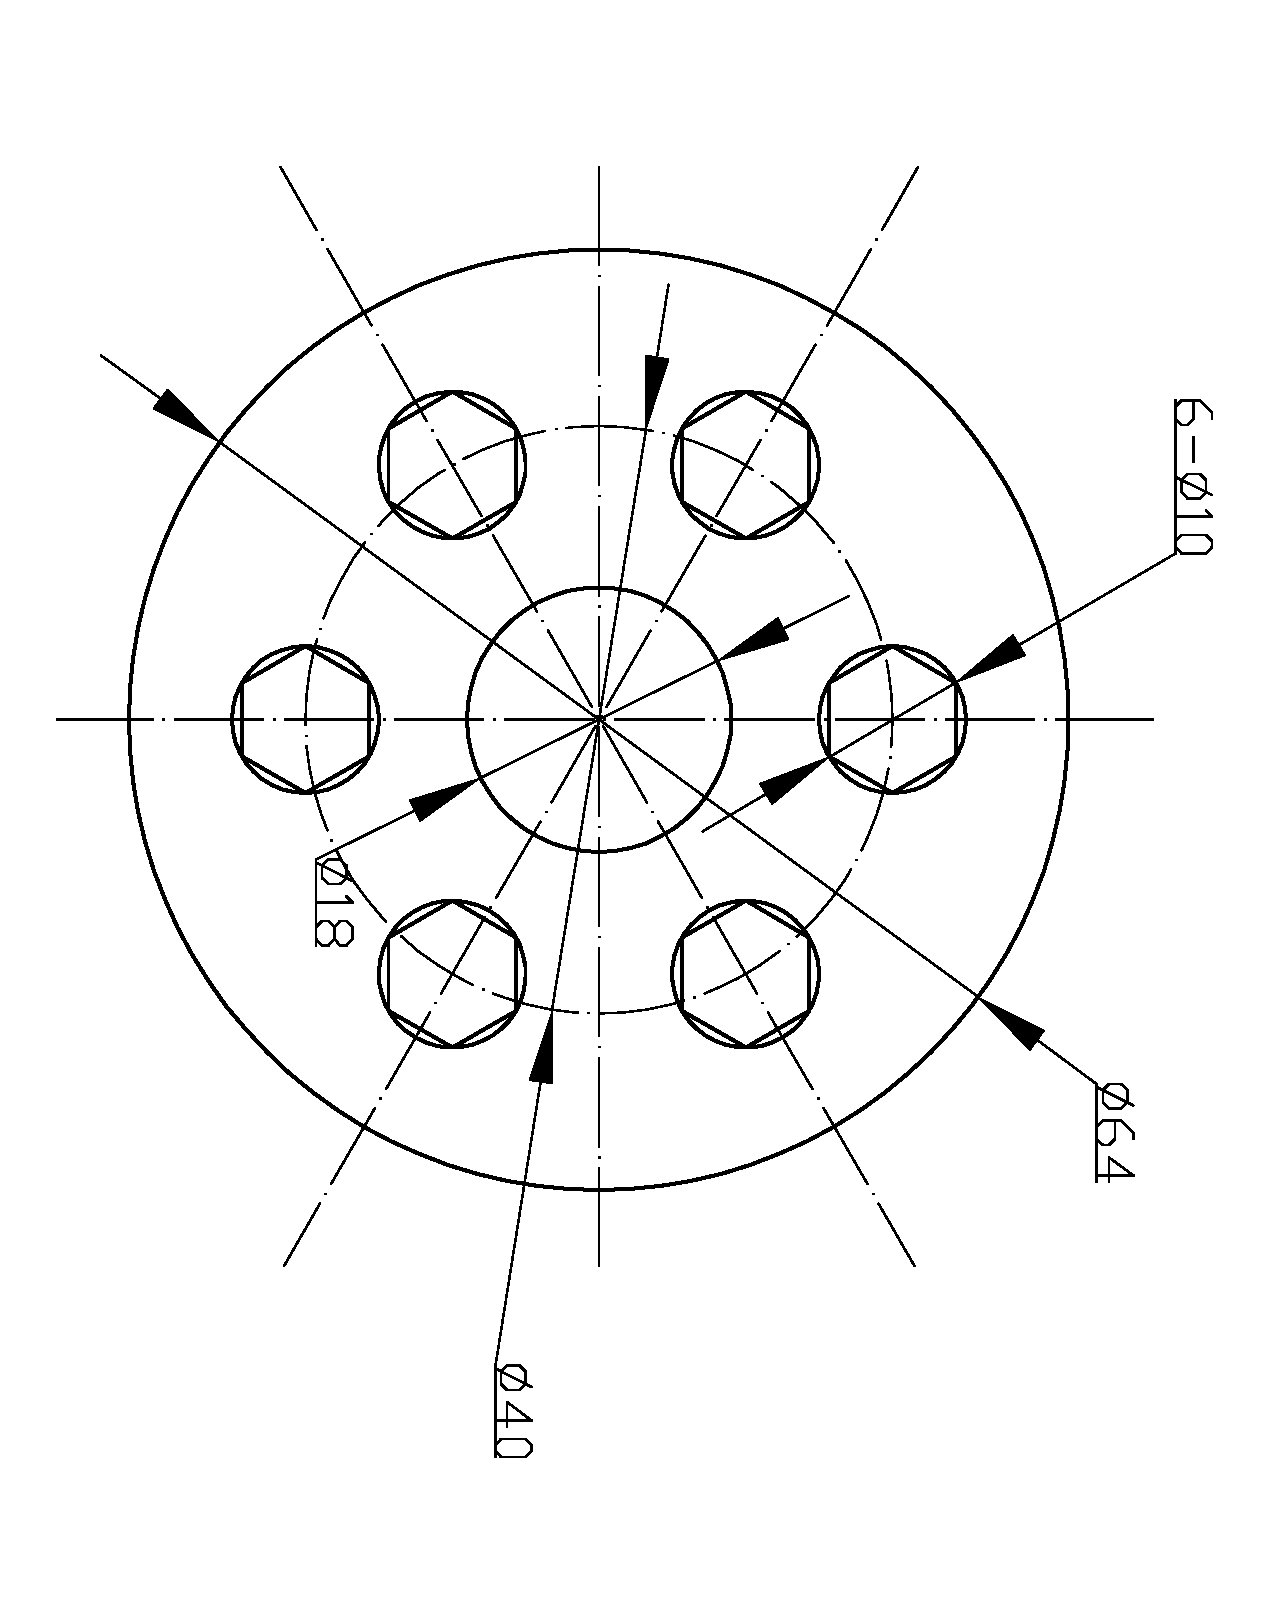
\includegraphics[scale=0.45,angle=90]{shu2.pdf}
\caption{任务二示例}\label{fig:renwu2}
\end{figure}

\indent
本任务以完成\ref{fig:renwu2}所示法兰盘图形为目标,旨在让读者掌握用AutoCAD的图层来管理各种图线,并学会构造线、圆、多边形和图形阵列编辑命令的使用技巧。并让读者认识和理解图样抄画的步骤和顺序,形成图样绘制的基本职业习惯。

\subsection{图层设置与管理}
\subsection{绘制图样}
\endinput

\chapter{绘制垫片立体图}\label{chap:dianpian}
第二天晚上秦奋满脸微笑地来到父亲的书房。他父亲见他兴趣盎然,说道:看来你的收获不错,把你绘的立体图给我检验一下。

秦奋将白天画的立体一一打开给父亲看。他父亲看了后非常满意,于是又问道:你说说旋转建模法和拉伸建模法的区别。

秦奋:旋转建模法只适合回转体类零件的建模,而拉伸建模法不仅可以用于回转体类块零件的建模,也可以用于平面体类零件的建模。

爸爸:说得很对,你已经把两种方法的精髓都掌握了。

秦奋:我们今天学习什么零件的建模呢?

爸爸拿出一幅调压阀垫片零件图(图\ref{fig:tiaoyafadianpian}说道:我们今天学习垫片零件的三维建模。

\noindent
\begin{figure}[htbp]
\centering
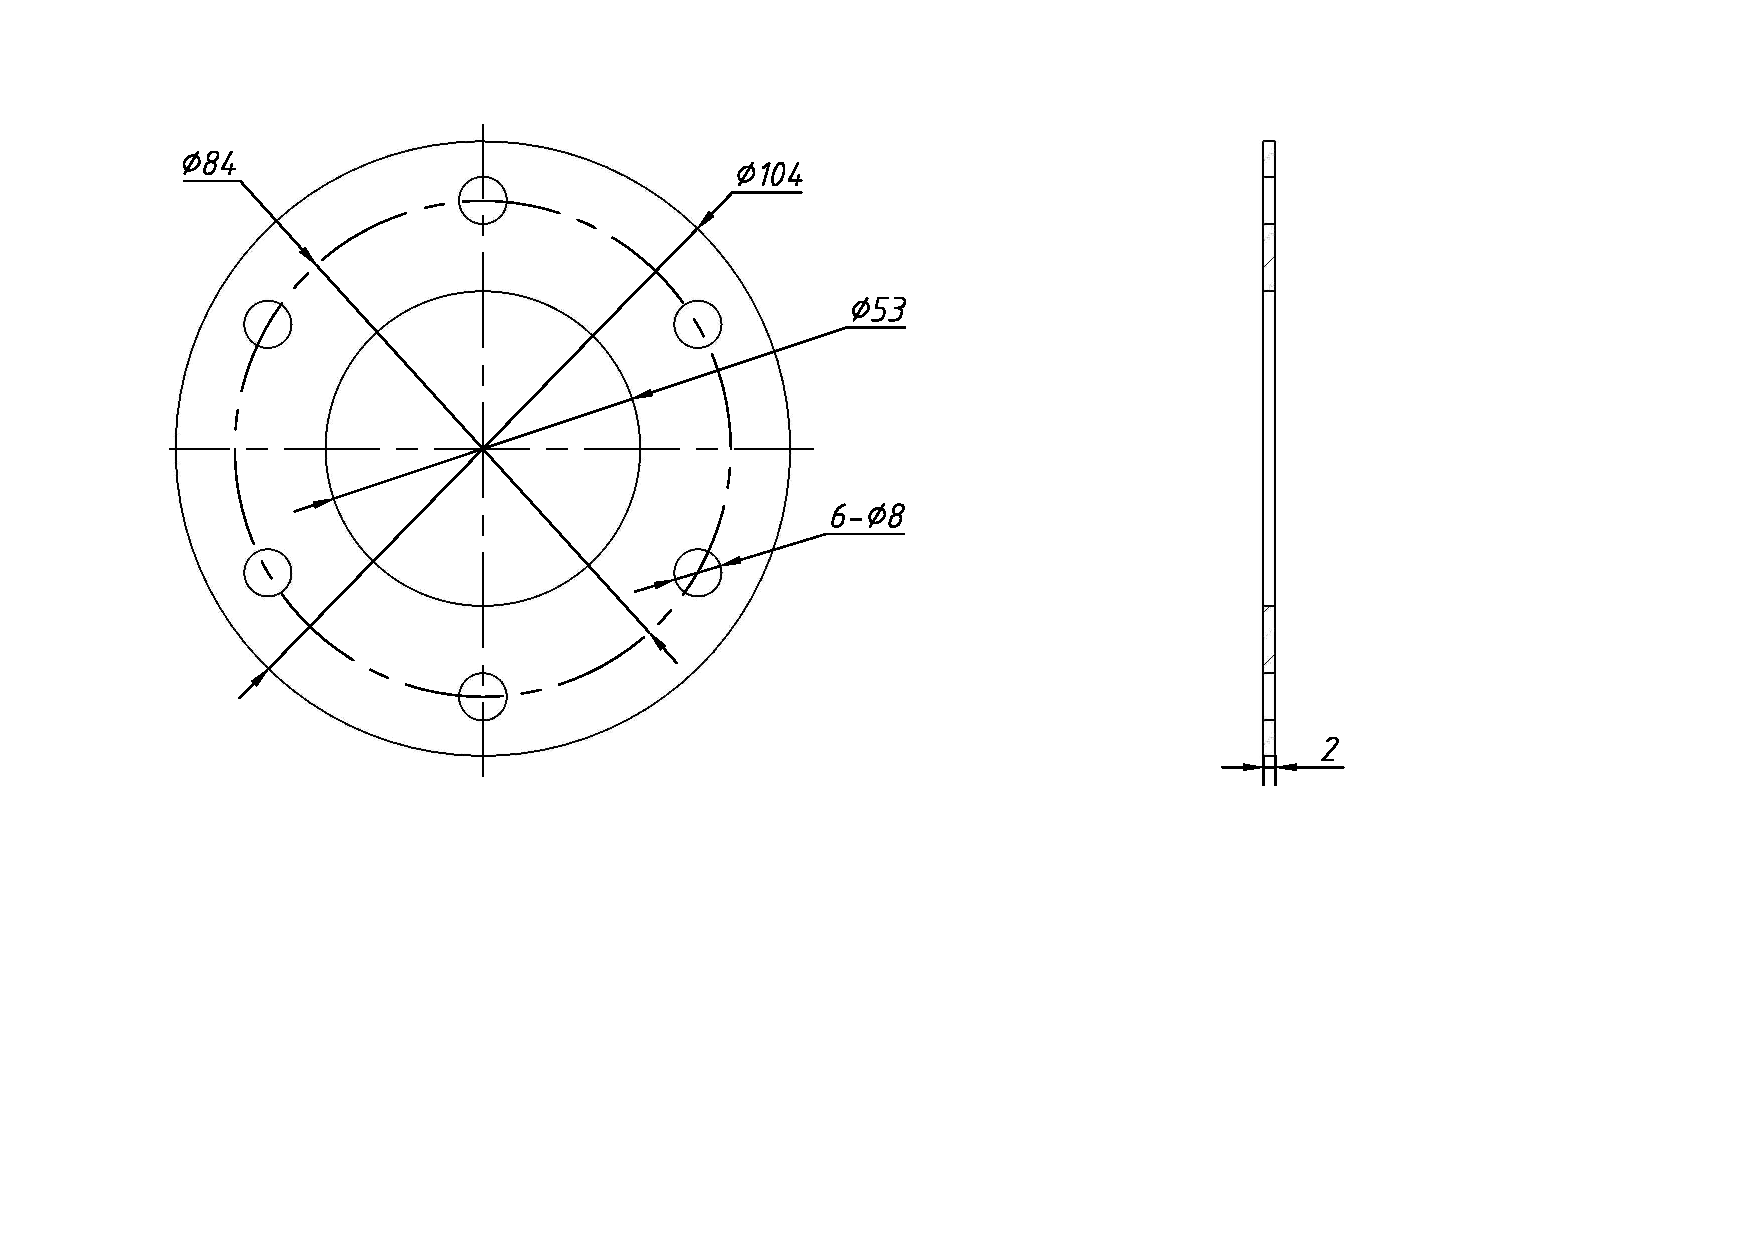
\includegraphics[scale=0.6]{tiaoyafadianpian.pdf}
\caption{垫片零件图}\label{fig:tiaoyafadianpian}
\end{figure}

秦奋看着零件图,皱眉道:昨天的零件图比较简单,图上所标注的尺寸关系我能够看懂,但今天的明显要困难一些。

爸爸:以后,我们将面对更加复杂的图形,其尺寸关系更加复杂,因此我们今天先了解平面图形分析方面的知识。
\endinput
\chapter{构建阀盖立三维模型}

{\bfseries 学习目标}
\begin{itemize}
\item 学习利用xline命令的角度选项绘制图形
\item 学习利用arc命令绘图形
\item 学习利用union命令构建三维模型
\item 学习利用创建布局向导创建布局
\item 掌握基本几何体的三视图表达
\item 学习利用viewbase命令生成基本视图
\end{itemize}

{\bfseries 任务要求}
\begin{itemize}
\item 根据图\ref{fig:tiaoyafafagai}所示的杯零件图,用拉伸法建立调压阀阀盖零件的三维模型
\item 利用阀盖三维模型生成基本三视图
\end{itemize}

\noindent
\begin{figure}[htbp]
\centering
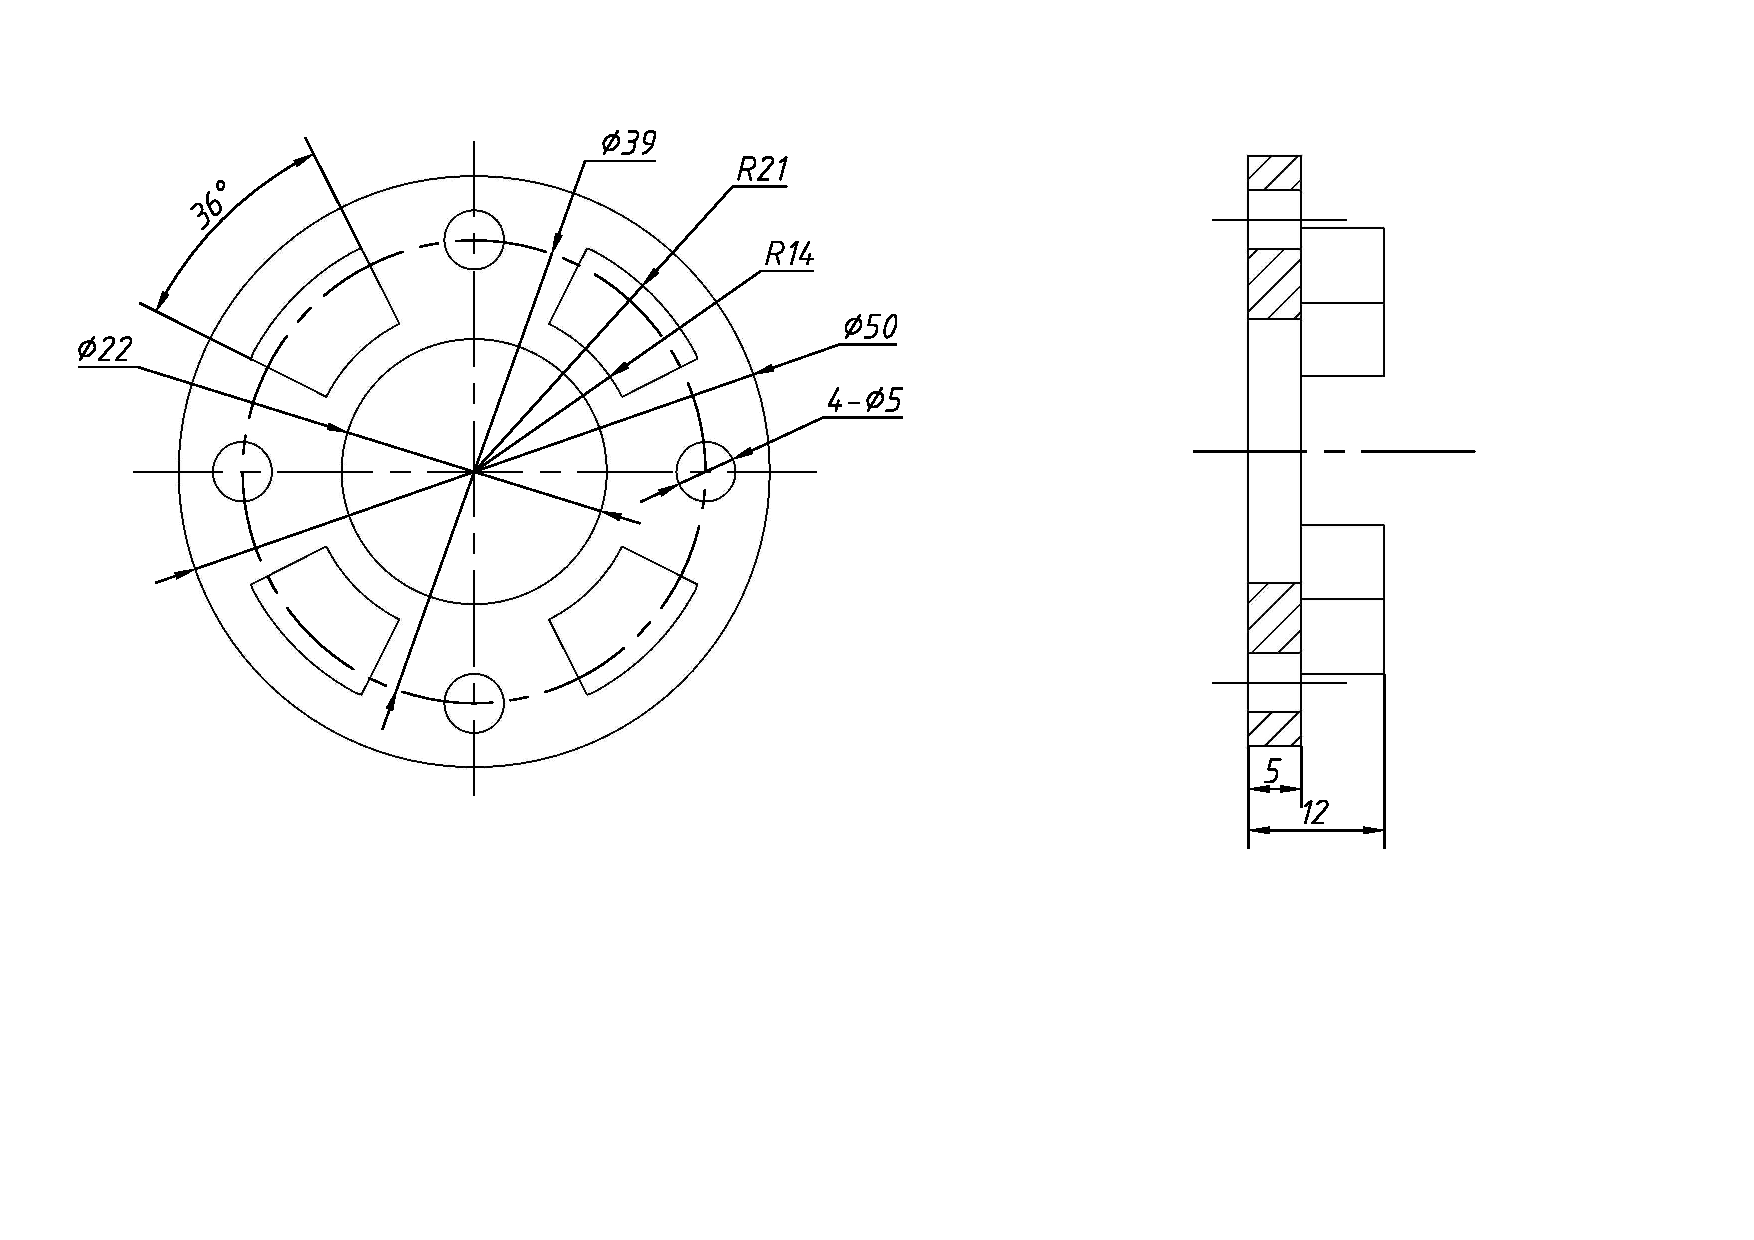
\includegraphics[scale=0.6]{tiaoyafafagai.pdf}
\caption{阀盖零件图}\label{fig:tiaoyafafagai}
\end{figure}
\clearpage

根据表面形状的不同可以将基本几何体分为平面立体和曲面立体。如果立体表面均由平面构成,则称为平面立体,如长方体、正方体、棱柱、棱锥、棱台等。如果立体表面由平面和曲面共同构成或全部由曲面构成,则称为曲面立体,如圆柱、圆球、圆环等。
\subsection{平面立体}
在平面立体中,平面立体的表面是由若干个平面多边形构成的,多边形的边是平面立体的轮廓线,是平面立体两个平面的交线,当轮廓的投影可见时,用粗实线表示;不可见时,用虚线表示;当实线与虚线重合时,应当用粗实线表示。
\subsubsection{棱柱体}
棱柱体由顶面、底面及若干个侧棱面构成。棱柱体的各个侧棱相互平行,顶面和底面相互平行。如果棱柱的侧棱与顶面和底面垂直则称为直棱柱,否则称为斜棱柱。当直棱柱的顶面和底面为正多边形时则称为正棱柱。
\begin{figure}[htbp]
\centering
\subfloat[]{\label{fig:cube}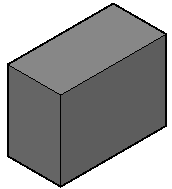
\includegraphics[scale=0.9]{cube.png}}\hspace{30pt}
\subfloat[]{\label{fig:cubethreeview}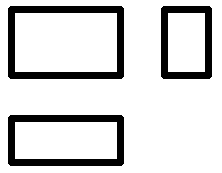
\includegraphics[scale=1]{cubethreeview.png}}
\caption{长方体的投影}
\end{figure}

图\ref{fig:cubethreeview}所示的长方体,其顶面与底面的水平投影重合并反映衬形,为一长方形,其它棱面的水平投影积聚为长方形的四条边;前面与后面的正投影重合并反映实形,顶面、底面和两个侧面积聚为长方形的四条件边;左面和右面的侧面投影重合并反映实形,顶面、底面、前面和后面积聚为长方形的四条件边。长方体的三视图投影如图\ref{fig:cube}所示。

图\ref{fig:sannenzhu}所示的正三棱柱,其顶面与底面的水平面投影重合并反映实形,为一正三角形。三个棱面在水平投影面积聚为三角形的三条边。三棱柱的三视图投影如图\ref{fig:sannenzhuthreeview}所示。
\begin{figure}[htbp]
\centering
\subfloat[]{\label{fig:sannenzhu}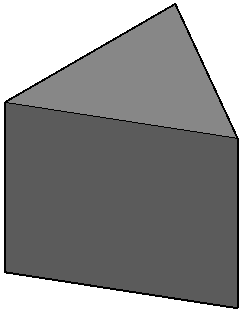
\includegraphics[scale=0.6]{sannenzhu.png}}\hspace{30pt}
\subfloat[]{\label{fig:sannenzhuthreeview}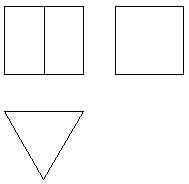
\includegraphics[scale=1]{sannenzhuthreeview.png}}
\caption{正三棱柱的投影}
\end{figure}

图\ref{fig:sixnenzhu}所示的正六棱柱,其顶面与底面的水平面投影重合并反映实形,为一正六边形。六个棱面在水平投影面积聚为六边形的六条边。正六棱柱的三视较长投影如图\ref{fig:sixnenthreeview}所示。
\begin{figure}[htbp]
\centering
\subfloat[]{\label{fig:sixnenzhu}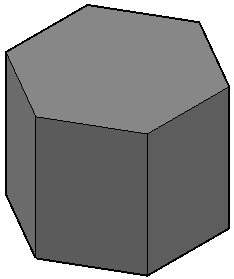
\includegraphics[scale=0.7]{sixnenzhu.png}}\hspace{30pt}
\subfloat[]{\label{fig:sixnenthreeview}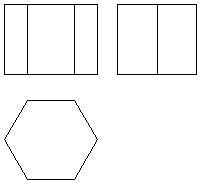
\includegraphics[scale=1]{sixnenthreeview.png}}
\caption{正六棱柱的投影}
\end{figure}

由此可见棱柱体的投影特点是:一面投影反映底面实形,其余两面投影则为矩形或复合矩形。
\subsubsection{棱锥体}
棱锥体是由一个多边形底面和若干个共顶点的三角形棱面构成的。从棱锥体顶点到底面的垂直距离称为棱锥体的高。如果棱锥体的底面为正多边形,锥顶的投影位于多边形的中心,各棱面是等腰三角形,则该棱锥体称为正棱锥。正四棱锥的三面投影如图\ref{fig:fournenzhuithreeview}所示。

\begin{figure}[htbp]
\centering
\subfloat[]{\label{fig:fournengzhui}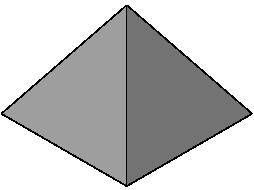
\includegraphics[scale=0.9]{fournengzhui.png}}\hspace{30pt}
\subfloat[]{\label{fig:fournenzhuithreeview}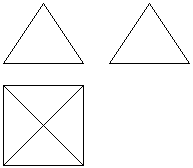
\includegraphics[scale=1]{fournenzhuithreeview.png}}
\caption{正四棱锥的投影}
\end{figure}

图\ref{fig:fournengzhui}所示的正四棱锥的底面与水平投影面平行,其投影反映实形,为正方形;底面在其它投影面积聚为一条直线;棱面的三面投影则为类似的三角形。

由此可见,棱锥体的投影特点是:一投影面为由三角形构成的复合多边形,其两投影为三角形或复合三角形。
\subsubsection{棱台体}
棱台体是由棱锥体被切掉顶部后所构成的一种形体。棱台体的投影特点是:一面投影为由梯形构成的内外相似复合多边形,其余两面投影则为梯形或复合梯形。图\ref{fig:fivenentai} 所示为五棱台的投影。
\begin{figure}[htbp]
\centering
\subfloat[]{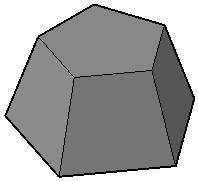
\includegraphics[scale=0.9]{fivenentai.png}}\hspace{30pt}
\subfloat[]{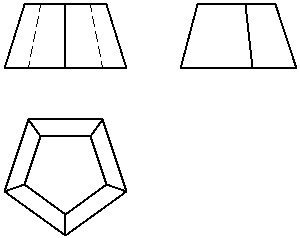
\includegraphics[scale=1]{fivenentaithreeview.png}}
\caption{五棱台的投影}\label{fig:fivenentai}
\end{figure}

\endinput
\subsection{曲面立体}
曲面体是由面或曲面和平面共同构成的立体,其中最常见的是回转曲面。回转体曲面是由一母线绕一空间轴线作旋转运动而形成的光滑曲面。母线在在回转曲面上任意位置称作素线,母线上任意一点的旋转轨迹都是一个圆,该圆称为纬圆。图\ref{fig:huizhuangti}所示为回转体的形成和术语。
\begin{figure}[htbp]
\centering
\subfloat[]{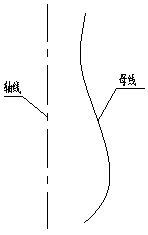
\includegraphics[scale=0.5]{huizhuangti.png}}\hspace{30pt}
\subfloat[]{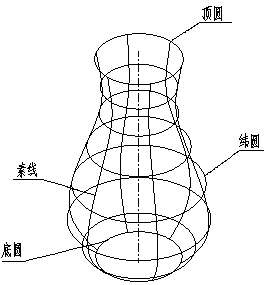
\includegraphics[scale=0.5]{rotatetree.png}}
\caption{回转体的形成及术语}\label{fig:huizhuangti}
\end{figure}

画回转体的投影图时,首先画出回转轴线,然后画出反映实形的投影,最后画其余两个投影。回转曲面向某一投影面投影时,轮廓素线是回转曲面在该投影面上可见和不可见面的分界线的投影,在分界线之前的回转曲面为可见,反之则不可见。画图时,凡不属于该投影面的轮廓素线,一律不画出。
\subsubsection{圆柱体}
圆柱体是由圆柱面、顶面、底面所构成的。圆柱体可以看作一条与轴线平行的母线绕轴线旋转而成的。图所示圆柱体的轴线垂直于水平投影面,其水平投影为圆;其正投影和侧投影均为矩形。
\begin{figure}[htbp]
\centering
\subfloat[]{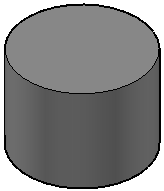
\includegraphics[scale=0.9]{yuanzhuti.png}}\hspace{30pt}
\subfloat[]{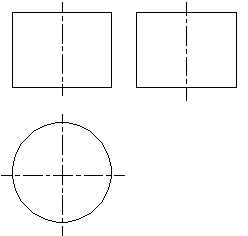
\includegraphics[scale=0.7]{yuanzhutithreeview.png}}
\caption{圆柱体的投影}\label{fig:yuanzhuti}
\end{figure}
\subsubsection{圆锥体}
图\ref{fig:yuanzhuiti} 所示的圆锥体底面与水平投影面平行,其投影为一圆,反映实形,在其余两个投影面上积聚为一条直线;圆锥体的其余两面投影均为等腰三角形。
\begin{figure}[htbp]
\centering
\subfloat[]{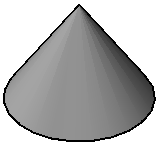
\includegraphics[scale=1]{yuanzhuiti.png}}\hspace{30pt}
\subfloat[]{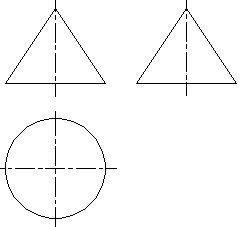
\includegraphics[scale=0.7]{yuanzhuitithreeview.png}}
\caption{圆锥体的投影}\label{fig:yuanzhuiti}
\end{figure}
\subsubsection{球体}
球体是由圆形母线以其直径为回转轴旋转而成的。球体的三面投影均为圆。
\begin{figure}[htbp]
\centering
\subfloat[]{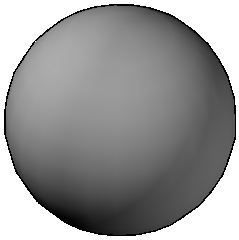
\includegraphics[scale=0.7]{qiouti.png}}\hspace{30pt}
\subfloat[]{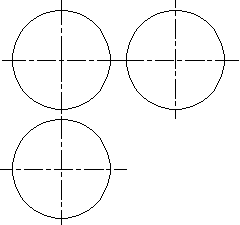
\includegraphics[scale=0.7]{qioutithreeview.png}}
\caption{球体的投影}\label{fig:qiout}
\end{figure}
\endinput
\section{法兰盘三视图}

{\bfseries 知识目标}
\begin{itemize}
\item 掌握回转体三视图规律
\end{itemize}

{\bfseries 技能目标}
\begin{itemize}
\item 能够应用三视图对应关系,运用AutoCAD绘制回转体的三视图
\end{itemize}

图\ref{fig:falanpanlititu}所示为工业中应用泛用于管道连接的法兰盘零件的简化形式。本任务主要是让读者了解并掌握回转体三视图表述方式,实现应用AutoCAD进行回转体类零件的三视图绘制的技能目标。
\begin{figure}[htbp]
\centering
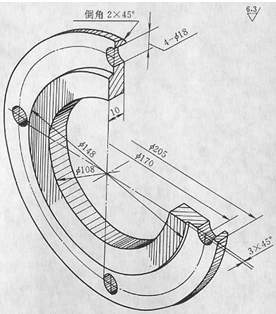
\includegraphics[scale=1]{fananlititu.png}
\caption{法兰盘}\label{fig:falanpanlititu}
\end{figure}
\subsection{绘制法兰盘主视图}
法兰盘整体是由两个圆筒叠加构成的,并具有四个用于安装的联接孔。我们先选择最能够表达的其形状的特征的方向作为其主视图。

具体绘图过程如下:

第一步:先定义图层,如图\ref{fig:falantucen}所示。
\begin{figure}[htbp]
\centering
\begin{floatrow}
\ffigbox{\caption{法兰盘图层定义}\label{fig:falantucen}}
{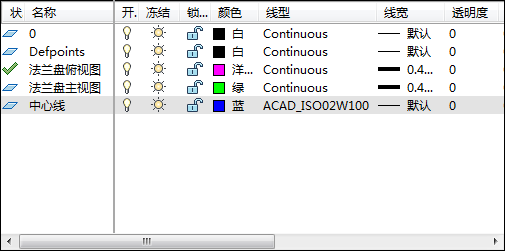
\includegraphics[scale=0.5]{falantucen.png}}
\ffigbox{\caption{法兰盘主视图}\label{fig:falanzhushitu}}{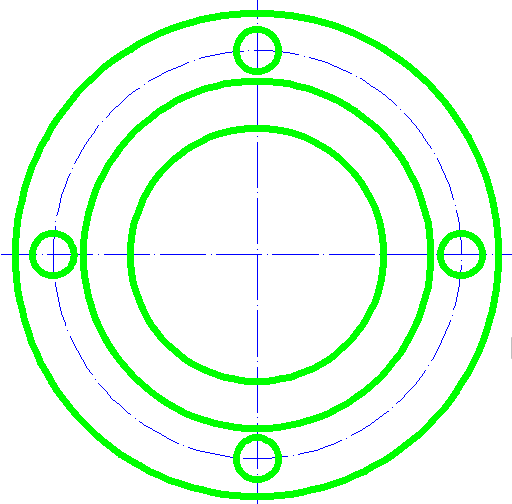
\includegraphics[scale=0.25]{falanzhushitu.png}}
\end{floatrow}
\end{figure}

第二步:绘制中心线,并完成主视图,如图\ref{fig:falanzhushitu}所示。

\begin{lstlisting}
%命令: line 指定第一点:%
%指定下一点或 [放弃(U)]: $@212<0$%
%指定下一点或 [放弃(U)]:%
%命令: LINE%
%指定第一点: @-106,106%
%指定下一点或 [放弃(U)]:$ @212<-90$%
%指定下一点或 [放弃(U)]:%
%命令: circle% 
%指定圆的圆心或 [三点(3P)/两点(2P)/切点、切点、半径(T)]: int%
%于%
%指定圆的半径或 [直径(D)]: 103%
%命令: circle %
%指定圆的圆心或 [三点(3P)/两点(2P)/切点、切点、半径(T)]: int%
%于%
%指定圆的半径或 [直径(D)]:$ <103.0000>$: 87%
%指定圆的圆心或 [三点(3P)/两点(2P)/切点、切点、半径(T)]: int%
%于%
%指定圆的半径或 [直径(D)]:$ <87.0000>$: 74%
%指定圆的圆心或 [三点(3P)/两点(2P)/切点、切点、半径(T)]: int%
%于%
%指定圆的半径或 [直径(D)]:$ <74.0000>$: 54%
%指定圆的圆心或 [三点(3P)/两点(2P)/切点、切点、半径(T)]: int%
%于%
%指定圆的半径或 [直径(D)]:$ <54.0000>$: 9%
%命令: arraypolar%
%选择对象: 找到 1 个%
%选择对象:%
%类型 = 极轴  关联 = 是%
%指定阵列的中心点或 [基点(B)/旋转轴(A)]: int%
%于%
%输入项目数或 [项目间角度(A)/表达式(E)]$ <4>:$%
%指定填充角度(+=逆时针、-=顺时针)或 [表达式(EX)] $<360>$:%
%按 Enter 键接受或 [关联(AS)/基点(B)/项目(I)/项目间角度(A)/填充%
%角度(F)/行(ROW)/层(L)/旋转项目(ROT)/退出(X)] %
%$<$退出$>$:%
\end{lstlisting}
\subsection{绘制法兰盘俯视图}
第一步:先利用长对正关系,确定定俯视图中对应部件的投影关系。
\begin{lstlisting}
%命令: line 指定第一点:%
%指定下一点或 [放弃(U)]: $ <$正交 开$>$%
%指定下一点或 [放弃(U)]:%
%命令: offset%
%当前设置: 删除源=否  图层=源  OFFSETGAPTYPE=0%
%指定偏移距离或 [通过(T)/删除(E)/图层(L)] %<%通过%>%:  10%
%选择要偏移的对象,或 [退出(E)/放弃(U)] $<$退出$>$:%
%指定要偏移的那一侧上的点,或 [退出(E)/多个(M)/放弃(U)] $<$退出$>$:%
%选择要偏移的对象,或 [退出(E)/放弃(U)] $<$退出$>$:%
%指定要偏移的那一侧上的点,或 [退出(E)/多个(M)/放弃(U)] $<$退出$>$:%
%选择要偏移的对象,或 [退出(E)/放弃(U)] $<$退出$>$:%
%命令: line %
%指定第一点: int%
%于%
%指定下一点或 [放弃(U)]: per%
%到%
%指定下一点或 [放弃(U)]:%
%命令: line %
%指定第一点: int%
%于%
%指定下一点或 [放弃(U)]: per%
%到%
%指定下一点或 [放弃(U)]:%
%命令: line %
%指定第一点: int%
%于%
%指定下一点或 [放弃(U)]: per%
%到%
%指定下一点或 [放弃(U)]:%
%命令: line %
%指定第一点: int%
%于%
%指定下一点或 [放弃(U)]: per%
%到%
%指定下一点或 [放弃(U)]:%
%命令: line %
%指定第一点: int%
%于%
%指定下一点或 [放弃(U)]: per%
%到%
%指定下一点或 [放弃(U)]:%
%命令: line %
%指定第一点: int%
%于%
%指定下一点或 [放弃(U)]: per%
%到%
%指定下一点或 [放弃(U)]:%
%命令: line %
%指定第一点: int%
%于%
%指定下一点或 [放弃(U)]: per%
%到%
%指定下一点或 [放弃(U)]:%
%命令: line %
%指定第一点: int%
%于%
%指定下一点或 [放弃(U)]: per%
%到%
%指定下一点或 [放弃(U)]:%
%命令: line %
%指定第一点: int%
%于%
%指定下一点或 [放弃(U)]: per%
%到%
%指定下一点或 [放弃(U)]:%
%命令: line %
%指定第一点: int%
%于%
%指定下一点或 [放弃(U)]: per%
%到%
%指定下一点或 [放弃(U)]:%
%命令: line %
%指定第一点: int%
%于%
%指定下一点或 [放弃(U)]: per%
%到%
%指定下一点或 [放弃(U)]:%
%命令: line %
%指定第一点: int%
%于%
%指定下一点或 [放弃(U)]: per%
%到%
%指定下一点或 [放弃(U)]:%
\end{lstlisting}

\begin{figure}[htbp]
\centering
\begin{floatrow}
\ffigbox{\caption{法兰盘俯视图}\label{fig:falanfushitu}}{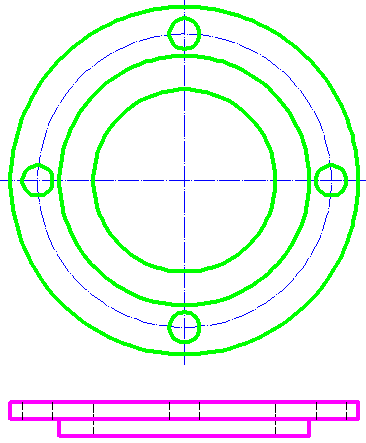
\includegraphics[scale=0.3]{falanfushitu.png}}
\ffigbox{\caption{法兰盘三视图}\label{fig:falansanshitu}}{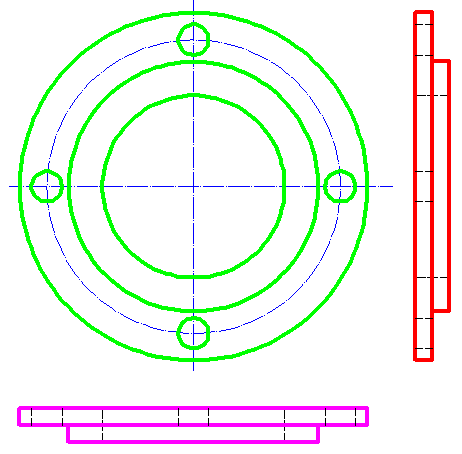
\includegraphics[scale=0.3]{falansanshitu.png}}
\end{floatrow}
\end{figure}

第二步:根据\ref{fig:falanpanlititu}所示尺寸绘出俯视图,如图\ref{fig:falanfushitu}所示。
\begin{lstlisting}
%命令: trim%
%当前设置:投影=UCS,边=无%
%选择剪切边...%
%选择对象或 $<$全部选择$>$:  找到 1 个%
%选择对象:%
%选择要修剪的对象,或按住 Shift 键选择要延伸的对象,或%
%[栏选(F)/窗交(C)/投影(P)/边(E)/删除(R)/放弃(U)]:  指定对角点:%
%选择要修剪的对象,或按住 Shift 键选择要延伸的对象,或%
%[栏选(F)/窗交(C)/投影(P)/边(E)/删除(R)/放弃(U)]:%
%命令: trim%
%当前设置:投影=UCS,边=无%
%选择剪切边...%
%选择对象或 $<$全部选择$>$:  找到 1 个%
%选择对象: 找到 1 个,总计 2 个%
%选择对象: 找到 1 个,总计 3 个%
%选择对象: 找到 1 个,总计 4 个%
%选择对象:%
%选择要修剪的对象,或按住 Shift 键选择要延伸的对象,或%
%[栏选(F)/窗交(C)/投影(P)/边(E)/删除(R)/放弃(U)]:  指定对角点:%
%选择要修剪的对象,或按住 Shift 键选择要延伸的对象,或%
%[栏选(F)/窗交(C)/投影(P)/边(E)/删除(R)/放弃(U)]:  指定对角点:%
%选择要修剪的对象,或按住 Shift 键选择要延伸的对象,或%
%[栏选(F)/窗交(C)/投影(P)/边(E)/删除(R)/放弃(U)]:%
%命令: TRIM%
%当前设置:投影=UCS,边=无%
%选择剪切边...%
%选择对象或 $<$全部选择$>$:  找到 1 个%
%选择对象:%
%选择要修剪的对象,或按住 Shift 键选择要延伸的对象,或%
%[栏选(F)/窗交(C)/投影(P)/边(E)/删除(R)/放弃(U)]:%
%选择要修剪的对象,或按住 Shift 键选择要延伸的对象,或%
%[栏选(F)/窗交(C)/投影(P)/边(E)/删除(R)/放弃(U)]:%
%选择要修剪的对象,或按住 Shift 键选择要延伸的对象,或%
%[栏选(F)/窗交(C)/投影(P)/边(E)/删除(R)/放弃(U)]:%
\end{lstlisting}

\subsection{绘制法兰盘左视图}
利用主、左高平齐,俯左宽相等的对应关系绘制左视图的相关部分,最终形成三视图如图\ref{fig:falansanshitu}所示。
\begin{lstlisting}
%命令: line 指定第一点:%
%指定下一点或 [放弃(U)]: $ <$正交 开$>$%
%指定下一点或 [放弃(U)]:%
%命令: offset%
%当前设置: 删除源=否  图层=源  OFFSETGAPTYPE=0%
%指定偏移距离或 [通过(T)/删除(E)/图层(L)] $<10.0000>$:  int%
%于  指定第二点: int%
%于%
%选择要偏移的对象,或 [退出(E)/放弃(U)] $<$退出$>$:%
%指定要偏移的那一侧上的点,或 [退出(E)/多个(M)/放弃(U)] $<$退出$>$:%
%选择要偏移的对象,或 [退出(E)/放弃(U)] $<$退出$>$:%
%命令: offset%
%当前设置: 删除源=否  图层=源  OFFSETGAPTYPE=0%
%指定偏移距离或 [通过(T)/删除(E)/图层(L)]$ <10.0000>$:  int%
%于  指定第二点: int%
%于%
%选择要偏移的对象,或 [退出(E)/放弃(U)] $<$退出$>$:%
%指定要偏移的那一侧上的点,或 [退出(E)/多个(M)/放弃(U)] $<$退出$>$:%
%选择要偏移的对象,或 [退出(E)/放弃(U)] $<$退出$>$:%
%命令: line %
%指定第一点: int%
%于%
%指定下一点或 [放弃(U)]: per%
%到%
%指定下一点或 [放弃(U)]:%
%命令: line %
%指定第一点: int%
%于%
%指定下一点或 [放弃(U)]: per%
%到%
%指定下一点或 [放弃(U)]:%
%命令: line %
%指定第一点: int%
%于%
%指定下一点或 [放弃(U)]: per%
%到%
%指定下一点或 [放弃(U)]:%
%命令: line %
%指定第一点: int%
%于%
%指定下一点或 [放弃(U)]: per%
%到%
%指定下一点或 [放弃(U)]:%
%命令: line %
%指定第一点: int%
%于%
%指定下一点或 [放弃(U)]: per%
%到%
%指定下一点或 [放弃(U)]:%
%命令: line %
%指定第一点: int%
%于%
%指定下一点或 [放弃(U)]: per%
%到%
%指定下一点或 [放弃(U)]:%
%命令: line %
%指定第一点: int%
%于%
%指定下一点或 [放弃(U)]: per%
%到%
%指定下一点或 [放弃(U)]:%
%命令: line %
%指定第一点: int%
%于%
%指定下一点或 [放弃(U)]: per%
%到%
%指定下一点或 [放弃(U)]:%
%命令: line %
%指定第一点: int%
%于%
%指定下一点或 [放弃(U)]: per%
%到%
%指定下一点或 [放弃(U)]:%
%命令: line %
%指定第一点: int%
%于%
%指定下一点或 [放弃(U)]: per%
%到%
%指定下一点或 [放弃(U)]:%
%命令: line %
%指定第一点: int%
%于%
%指定下一点或 [放弃(U)]: per%
%到%
%指定下一点或 [放弃(U)]:%
%命令: line %
%指定第一点: int%
%于%
%指定下一点或 [放弃(U)]: per%
%到%
%指定下一点或 [放弃(U)]:%
%命令: trim%
%当前设置:投影=UCS,边=无%
%选择剪切边...%
%选择对象或 $<$全部选择$>$:  找到 1 个%
%选择对象:%
%选择要修剪的对象,或按住 Shift 键选择要延伸的对象,或%
%[栏选(F)/窗交(C)/投影(P)/边(E)/删除(R)/放弃(U)]:  指定对角点:%
%选择要修剪的对象,或按住 Shift 键选择要延伸的对象,或%
%[栏选(F)/窗交(C)/投影(P)/边(E)/删除(R)/放弃(U)]:%
%命令: trim%
%当前设置:投影=UCS,边=无%
%选择剪切边...%
%选择对象或 $<$全部选择$>$:  找到 1 个%
%选择对象: 找到 1 个,总计 2 个%
%选择对象: 找到 1 个,总计 3 个%
%选择对象: 找到 1 个,总计 4 个%
%选择对象:%
%选择要修剪的对象,或按住 Shift 键选择要延伸的对象,或%
%[栏选(F)/窗交(C)/投影(P)/边(E)/删除(R)/放弃(U)]:  指定对角点:%
%选择要修剪的对象,或按住 Shift 键选择要延伸的对象,或%
%[栏选(F)/窗交(C)/投影(P)/边(E)/删除(R)/放弃(U)]:  指定对角点:%
%选择要修剪的对象,或按住 Shift 键选择要延伸的对象,或%
%[栏选(F)/窗交(C)/投影(P)/边(E)/删除(R)/放弃(U)]:%
%命令: TRIM%
%当前设置:投影=UCS,边=无%
%选择剪切边...%
%选择对象或 $<$全部选择$>$:  找到 1 个%
%选择对象:%
%选择要修剪的对象,或按住 Shift 键选择要延伸的对象,或%
%[栏选(F)/窗交(C)/投影(P)/边(E)/删除(R)/放弃(U)]:%
%选择要修剪的对象,或按住 Shift 键选择要延伸的对象,或%
%[栏选(F)/窗交(C)/投影(P)/边(E)/删除(R)/放弃(U)]:%
%选择要修剪的对象,或按住 Shift 键选择要延伸的对象,或%
%[栏选(F)/窗交(C)/投影(P)/边(E)/删除(R)/放弃(U)]:%
\end{lstlisting}
\endinput
\section{轴承支座三视图}

\endinput
\section{生成阀盖三视图}
\begin{procedure}
\item 打开“调压阀阀盖立体图.dwg”文件,并另存为“调压阀阀盖布局图.dwg”。

这样做的目的是为了保护源文件,以防止误操作后可进行有效的恢复之前的工作。AutoCAD本身并没有要求这样做。
\item 新建布局。

新建布局的方法有:
\begin{itemize}
\item 键盘输入LAYEROUT命令中的【新建N】选项。
\item 点击【插入】菜单中【布局】子菜单中的【新建布局】项。
\item 点击【插入】菜单中【布局】子菜单中的【创建布局向导】项。
\item 右击【模型】和【布局】
\includegraphics[scale=0.8]{buju.png} 区域,在弹出菜单中选择【新建布局】项。
\item 单击【模型】和【布局】
\includegraphics[scale=0.8]{buju.png} 区域中的【布局1】或【布局2】选项卡。
\item 点击【布局】工具栏中的【新建布局图标】
\includegraphics[scale=0.7]{buju1.png}
\end{itemize}
在此我们以【创建布向导】的方式来讲述如何新建布局。启动【创建布局】向导后会弹出图\ref{fig:bujuxiangdao1}所示对话框。
\begin{figure}[htbp]
\centering
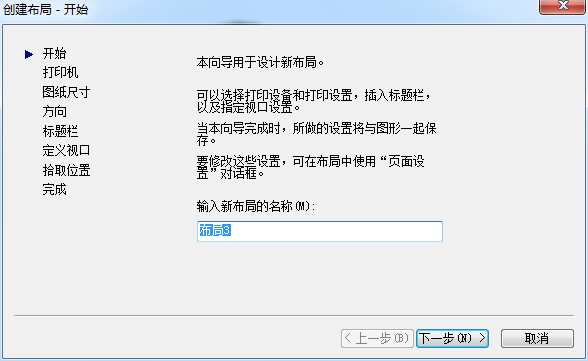
\includegraphics[scale=0.8]{bujuxiangdao1.png}
\caption{创建布局-开始对话框}\label{fig:bujuxiangdao1}
\end{figure}

此时,输入布局的名称并单下一步,弹出图\ref{fig:bujuxiangdao2}所示打印机设置对话框,将打印机设置为“DWG TO PDF.pc3"。实际工作中则就设置为可用的打印设备。
\begin{figure}[htbp]
\centering
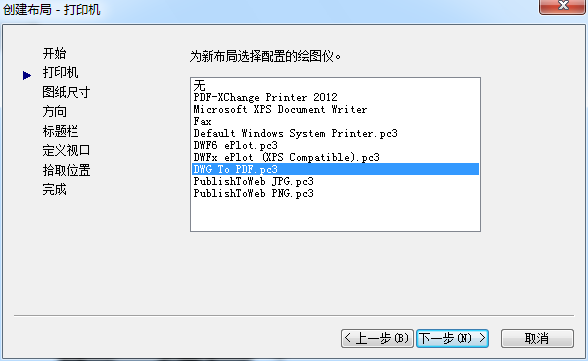
\includegraphics[scale=0.7]{bujuxiangdao2.png}
\caption{创建布局-打印机}\label{fig:bujuxiangdao2}
\end{figure}

设置完打印机后,单击下一步,弹出图\ref{fig:bujuxiangdao3}所示的图纸尺寸设置对话框。单击下拉框,将图纸设置为“ISO A4(297.00x210.00毫米)”,图形单位设置为毫米。
\begin{figure}[htbp]
\centering
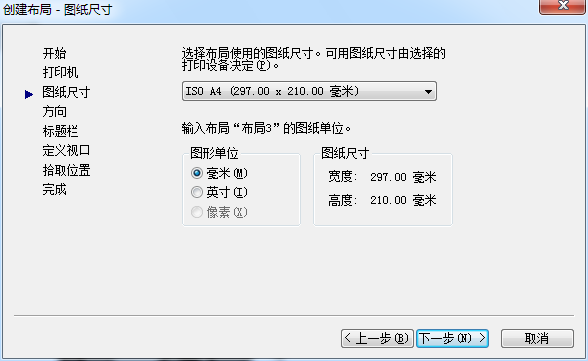
\includegraphics[scale=0.7]{bujuxiangdao3.png}
\caption{创建布局-图纸尺寸}\label{fig:bujuxiangdao3}
\end{figure}

设置完成后,单击下一步,弹出图\ref{fig:bujuxiangdao4}所示的方向设置对话框。此时将图形在图纸上的方向设置为横向。
\newpage
\begin{figure}[htbp]
\centering
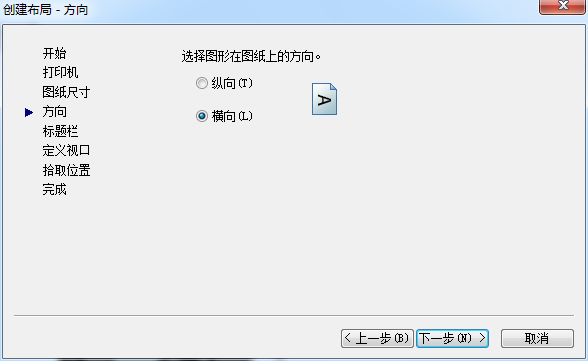
\includegraphics[scale=0.7]{bujuxiangdao4.png}
\caption{创建布局-方向}\label{fig:bujuxiangdao4}
\end{figure}

设置完成后,单击下一步,弹出图\ref{fig:bujuxiangdao5}所示的标题栏设置对话框。此时,将标题栏路径设置为无。
\begin{figure}[htbp]
\centering
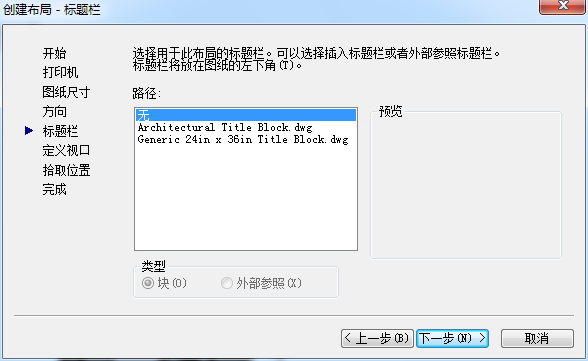
\includegraphics[scale=0.7]{bujuxiangdao5.png}
\caption{创建布局-标题栏}\label{fig:bujuxiangdao5}
\end{figure}

设置完成后,单击下一步,弹出图\ref{fig:bujuxiangdao6}所示的定义视口对话框。视口设置中单个表示创建一个视口,标准三维工程视图创建四个相等三个视口,阵列用于创建指定行和列的视口中。视口比例用于设置视口中显示对象的比例。由于生成三视图不需要用视口,因此在视口设置中选择无。
\newpage
\begin{figure}[htbp]
\centering
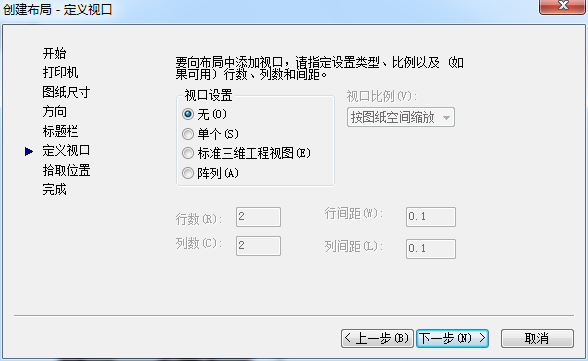
\includegraphics[scale=0.7]{bujuxiangdao6.png}
\caption{创建布局-定义视口}\label{fig:bujuxiangdao6}
\end{figure}

设置完成后,单击下一步,并点击完成,结束布局创建。
\item 从布局空间切换至模型空间。
\item 将工作空间由AutoCAD经典切换为三维建模,如图\ref{fig:sanweijianmo}所示。
\begin{figure}[htbp]
\centering
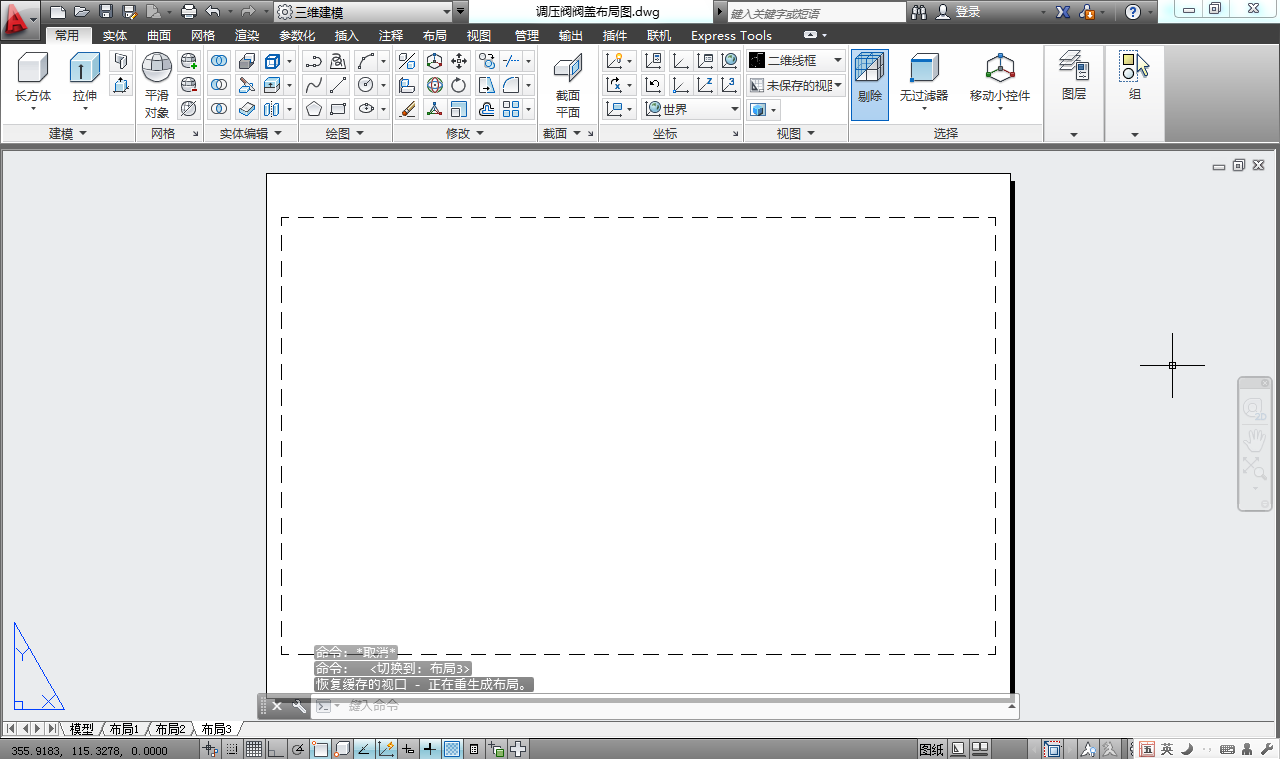
\includegraphics[scale=0.3]{sanweijianmo.png}
\caption{创建布局-定义视口}\label{fig:sanweijianmo}
\end{figure}
\item 创建基础视图。
启动创建基础视图的方法有:
\begin{itemize}
\item 键盘输出VIEWBASE。
\item 点【布局选项卡】中的【基础】图标
\includegraphics[scale=0.5]{viewbase.png},从下拉框中的选择
\includegraphics[scale=0.45]{comefrommodel.png}项
\end{itemize}
\newpage
启动命令后,选择从模式空间生成。
\begin{lstlisting}
|命令: VIEWBASE|
|指定模型源 [模型空间(M)/文件(F)] $<$模型空间$>$:
\end{lstlisting}
从模型空间中选择阀盖实体。
\begin{lstlisting}
|选择对象或 [整个模型(E)] $<$整个模型$>$: 找到 1 个|
|选择对象或 [整个模型(E)] $<$整个模型$>$:|
\end{lstlisting}
选择新创建的布局3作为生成的图纸。
\begin{lstlisting}
|输入要置为当前的新的或现有布局名称或 [?] $<$布局3$>$:|
|恢复缓存的视口 - 正在重生成布局。|
|命令:|
|类型 = 基础和投影  隐藏线 = 可见线和隐藏线  比例 = 1:1|
\end{lstlisting}
指定主视图的位置,如图\ref{fig:fagaibaseview1}所示。
\begin{lstlisting}
|指定基础视图的位置或 [类型(T)/选择(E)/方向(O)/隐藏线(H)/|
|比例(S)/可见性(V)] $<$类型$>$:|
|选择选项 [选择(E)/方向(O)/隐藏线(H)/比例(S)/可见性(V)/移动(M)|
|/退出(X)] $<$退出$>$:|
\end{lstlisting}
\begin{figure}[htbp]
\centering

\includegraphics[scale=1.4]{fagaibaseview1.png}
\caption{指定主视图位置}\label{fig:fagaibaseview1}
\end{figure}
选择左视图的投影视图位置
\begin{lstlisting}
|指定投影视图的位置或 $<$退出$>$:|
\end{lstlisting}
\begin{figure}[htbp]
\centering
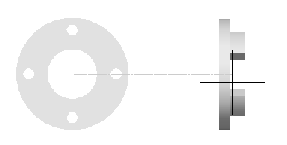
\includegraphics[scale=1.4]{fagaibaseview2.png}
\caption{指定左视图位置}\label{fig:fagaibaseview2}
\end{figure}
\newpage
选择俯视图的投影视图位置
\begin{lstlisting}
|指定投影视图的位置或 [放弃(U)/退出(X)] $<$退出$>$:|
|指定投影视图的位置或 [放弃(U)/退出(X)] $<$退出$>$:|
\end{lstlisting}
\begin{figure}[htbp]
\centering
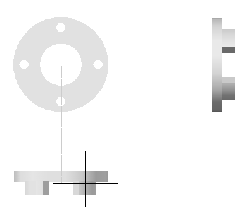
\includegraphics[scale=1.2]{fagaibaseview3.png}
\caption{指定左视图位置}\label{fig:fagaibaseview3}
\end{figure}
最终结果如图\ref{fig:fagaibaseview4} 所示。
\begin{figure}[htbp]
\centering
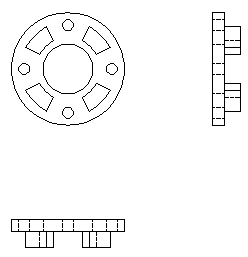
\includegraphics[scale=1.2]{fagaibaseview4.png}
\caption{阀盖三视图}\label{fig:fagaibaseview4}
\end{figure}
\end{procedure}
\endinput
\endinput
\chapter{构建端盖三维模型}\label{chap:duangai}

{\bfseries 学习目标}
\begin{itemize}
\item 学习利用fillet命令绘制连接圆弧
\item 学习利用filletedge命令构建三维圆弧
\end{itemize}

{\bfseries 任务要求}
\begin{itemize}
\item 根据图\ref{fig:tiaoyafaduangai}所示的杯零件图,用旋转法建立调压阀杯零件的三维模型
\item 根据图\ref{fig:tiaoyafaduangai}所示的杯零件图,用实体建模法建立调压阀杯零件的三维模型
\end{itemize}

\noindent
\begin{figure}[htbp]
\centering
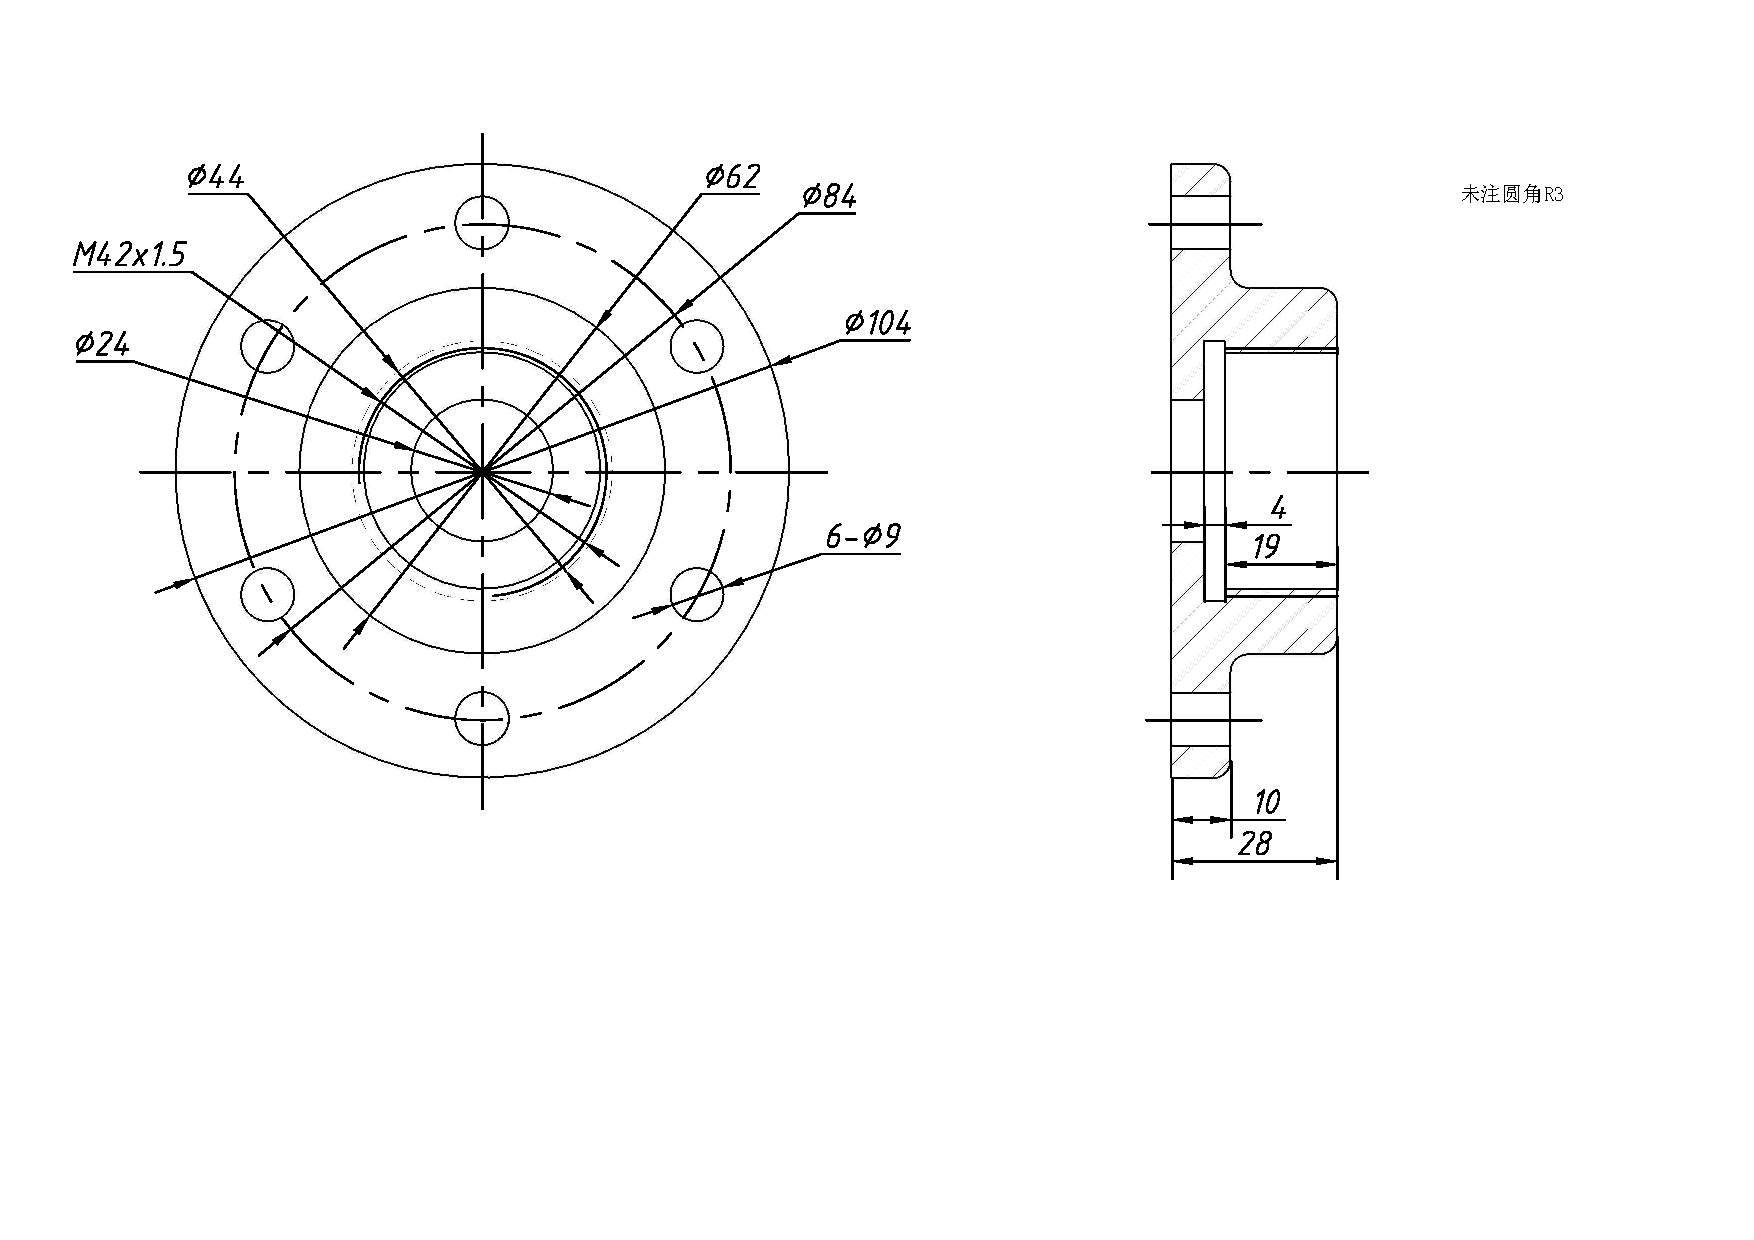
\includegraphics[scale=0.5]{tiaoyafaduangai.pdf}
\caption{端盖零件图}\label{fig:tiaoyafaduangai}
\end{figure}
\clearpage
\section{V型块立体图}

\endinput
\section{法兰盘立体图}

\endinput
\endinput
\chapter{构建阀体三维模型}

{\bfseries 学习目标}
\begin{itemize}
\item 学习利用chamfer命令绘制图形
\item 学习利用chamferedge命令建立三维倒角
\end{itemize}

{\bfseries 任务要求}
\begin{itemize}
\item 根据图\ref{fig:tiaoyafafati}所示的杯零件图,用旋转法建立调压阀阀体零件的三维模型
\end{itemize}

\noindent
\begin{figure}[htbp]
\centering
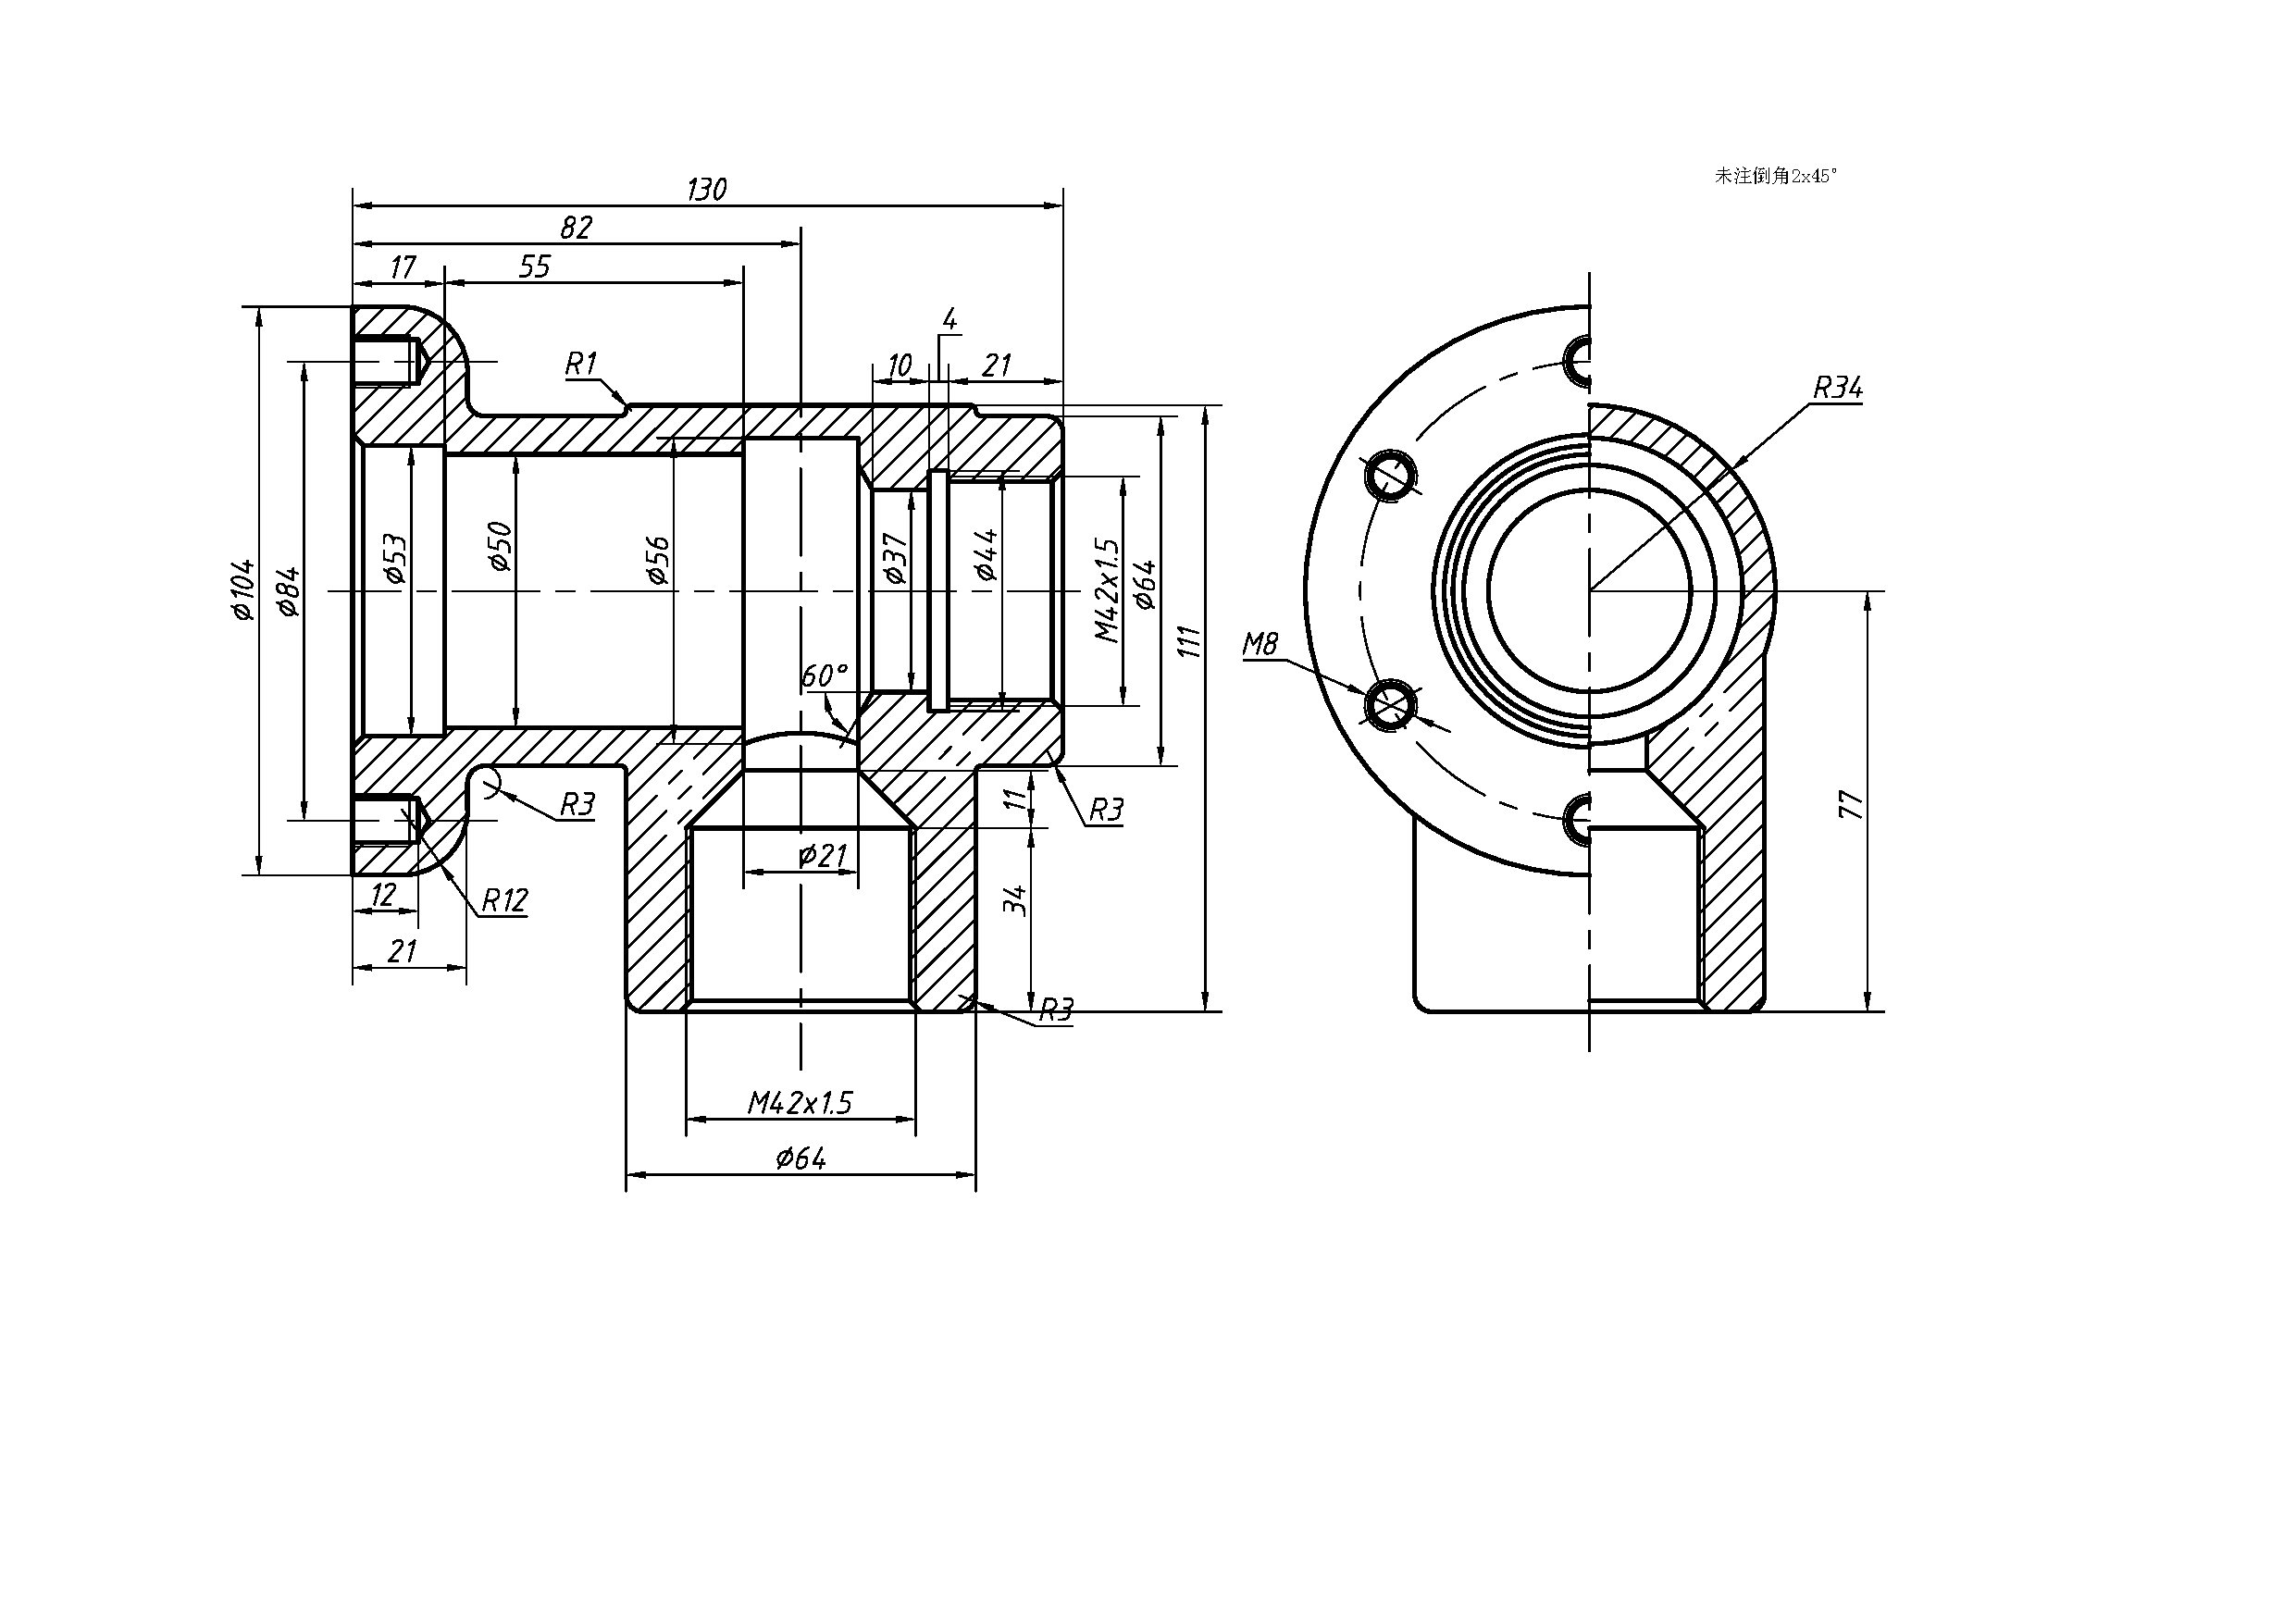
\includegraphics[scale=0.45]{tiaoyafafati.pdf}
\caption{阀体零件图}\label{fig:tiaoyafafati}
\end{figure}
\clearpage
\section{看组合体视图}
\subsection{识读要点}
\subsubsection{视图中线框和图形的理解}
一、视图中的每个线框,通常表示的是物体上一个表面(平面、曲面或平面和曲面相切)的投影。图\ref{fig:kantu8}中,线框A和E代表一个平面,线框F代表一个曲面,线框E代表平面和典相切。

二、视图中的相邻线框,表示物体上不同位置的两个表面。两个表面或是上下、左右、前后的位置关系,或者是两表面相交。图\ref{fig:kantu8}中,A、D两个面,A面在上,B面在下;A、D两个面,A面在右,D面在左。

\begin{figure}[htbp]
\centering
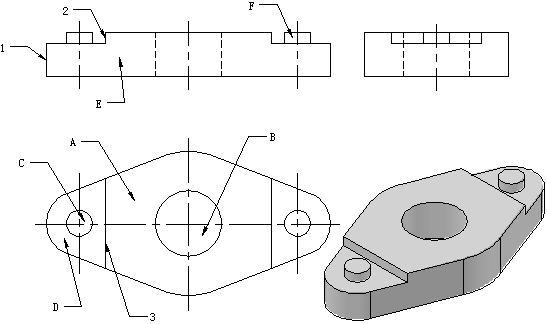
\includegraphics[scale=0.9]{kantu8.png}
\caption{线框和图形的含义}\label{fig:kantu8}
\end{figure}


三、视图中大线框套小线框,表示物体龙须面上凸出或凹进的关系。图\ref{fig:kantu8}中,C、D两个面,C为凸出;A、B两个面,B为凹进。

四、视图中的第一条线,可能是立体表面有积聚性表面的投影,如图\ref{fig:kantu8}中的线2;也可能是两平面的投影,如图\ref{fig:kantu8}中的线3;也可能是曲面转向轮廓线的投影,如图\ref{fig:kantu8}中的线1。
\subsubsection{联系多个视图进行识读}
在缺少尺寸瓢的情况下,一个视图是不能够确定物体的形状的。因为一个视图只能够表达两个方向的尺寸,一般不能够确切地表达出物体的三维空间形状。如图\ref{fig:kantu9}所示,如果仅仅只用主视图难以准确表达出物体的三维形状。根据俯视图的不同,物体的底板可能是倒角、凸字形和凹字形。因此,看图不能仅看一个或两个视图,而要把三个视图联系起来进行分析,才能够确定物体的形状。

\begin{figure}[htbp]
\centering
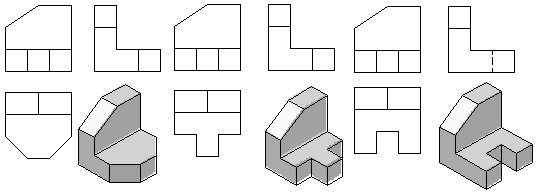
\includegraphics[scale=0.9]{kantu9.png}
\caption{一个视图不能确切地表达物体的形状}\label{fig:kantu9}
\end{figure}

如果视图选择不当,即使有两个视图也不能够准确地表达出物体的三维形状。如图\ref{fig:kantu9}所示,如果采用主视图和左视图就不能够清楚地表达出物体的形状。


\subsubsection{确定主特征视图}
特征视图是能够充分反映物体形状或相互位置特征的视图。特征视图通常分类形状特征视图和位置特征视图。形状特征图是能够充分反映物体形状特征的视图。图\ref{fig:kantu10}的主视图为形状特征视图,\ref{fig:kantu11}的俯视图为形状特征视图,它们都充分反映了特征的形状特征
\begin{figure}[htbp]
\centering
\subfloat[主视图为形状特征视图]{\label{fig:kantu10}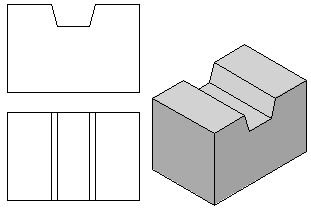
\includegraphics[scale=0.7]{kantu10.png}}\hspace{30pt}
\subfloat[俯视图为形状特征视图]{\label{fig:kantu11}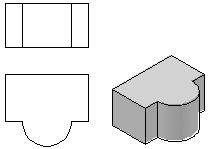
\includegraphics[scale=1]{kantu11.png}}
\caption{形状特征视图}
\end{figure}

位置特征图是能够充分反映相互位置特征的视图。图\ref{fig:kantu12}和\ref{fig:kantu13}所示的主视图是物体的形状特征图,但仅依靠主视图和俯视图不能够确定出1和2两个线框所代表的形状的具体位置。它们的左视图则清楚地反映方孔和圆柱的具体位置关系。
\begin{figure}[htbp]
\centering
\subfloat[]{\label{fig:kantu12}\includegraphics[scale=0.9]{kantu12.png}}\hspace{30pt}
\subfloat[]{\label{fig:kantu13}\includegraphics[scale=0.9]{kantu13.png}}
\caption{位置特征视图}
\end{figure}
\subsubsection{注意反映形体联接关系的图线}
形体之间的联接关系的变化,会导致视图中的图线产生相应的变化。图\ref{fig:kantu14}所示,三角形肋板与底板的连接是实线,说明它们的前面不是位于同一平面的错位关系,由俯视图可知三角形肋板位于底板中间。图\ref{fig:fati15}的中间是虚线连接,三角形肋板与底板的前面是位于同一个平面的,根据俯视图可以确定三角形肋板有两块,一块位于前面,另一块位于后面。
\begin{figure}[htbp]
\centering
\subfloat[]{\label{fig:kantu14}\includegraphics[scale=0.9]{kantu14.png}}\hspace{30pt}
\subfloat[]{\label{fig:kantu15}\includegraphics[scale=0.9]{kantu15.png}}
\caption{形体之间的表面联接关系}
\end{figure}
\endinput
\subsection{形体分析法}
形体分析法是从能够反映物体形状特征的视图出发,分析该物体由哪几个部分组成,采用什么形式组合,然后运用视图投影规律,找出每个部分在其它视图上的投影,从而想象出各个部分所表达的基本形体的形状及各部分之间的相互位置关系,最后综合想象出整个物体的形状的方法。

下面以图所示的三视图来说明形体分析法看图的步骤。

一、看视图,分析物体的形体组成部分。运用形体分析法将视图分成3个部分,如图\ref{fig:kantu}所示。
\begin{figure}[htbp]
\centering
\includegraphics[scale=0.5]{kantu.png}
\caption{分析组成部分}\label{fig:kantu}
\end{figure}

二、找投影关系,想形体。从线框出发,从三视图中找出各个部分的投影,确定特征视图,想象形状。
\begin{figure}[htbp]
\centering
\subfloat[]{\label{fig:kantu3}\includegraphics[scale=0.4]{kantu3.png}}\hspace{30pt}
\subfloat[]{\label{fig:kantu4}\includegraphics[scale=0.6]{kantu4.png}}
\caption{套筒部分}
\end{figure}

\begin{figure}[htbp]
\centering
\subfloat[]{\label{fig:kantu1}\includegraphics[scale=0.4]{kantu1.png}}\hspace{30pt}
\subfloat[]{\label{fig:kantu2}\includegraphics[scale=0.3]{kantu2.png}}
\caption{底板部分}
\end{figure}
图\ref{fig:kantu3}所示,粗实线为第1部分套筒的三视图,从三视图可知,该套筒上前部分开有缺口,左中部分开有孔,如图\ref{fig:kantu4}所示。

图\ref{fig:kantu1}所示,粗实线为第2部分底板的三视图,从三视图可知,该底板整体上为一凸台,并有三个通孔,如图\ref{fig:kantu2}所示。

图\ref{fig:kantu5}所示,粗实线为第三部分凸台的三视图,从三视可知,该凸台由四棱体和半圆柱构成,并且右边被圆柱曲面切割,上半部分有一通孔, 如图\ref{fig:kantu6}所示。

\begin{figure}[htbp]
\centering
\subfloat[]{\label{fig:kantu5}\includegraphics[scale=0.4]{kantu5.png}}\hspace{30pt}
\subfloat[]{\label{fig:kantu6}\includegraphics[scale=0.3]{kantu6.png}}
\caption{凸台部分}
\end{figure}

三、明确位置和连接关系。在想象出各部分形体后,需要利用位置特征视图,确定各部分的位置和表面连接关系。确定位置关系和表面连接关系通常是难以截然分开的,需要进行综合考虑。图\ref{fig:kantu}所示,第1部分位于第2部分上面正中心位置,第3部分位于第2部分上面,位于第1部分左边并与之相贯。

四、综合分析,想象整体。将上面各个部分的形体和位置分析综合起,便可以想角出整个形体,如图\ref{fig:kantu7}所示。
\begin{figure}[htbp]
\centering
\includegraphics[scale=1]{kantu7.png}
\caption{支座空间形体}\label{fig:kantu7}
\end{figure}
\endinput
%\subsection{线面分析法}
线面分析法是分析组合体视图中某些线、面的投影关系,运用线、面的投影特征,分析视图中每一条线或线框所代表的含义和位置关系,用以确定物体形状的方法。

下面以为例来说明线面分析法看图的基本步骤。


\endinput
\section{构建阀体三维模型}
\section{构建阀体三维模型}
\subsection{绘制阀体旋转矩形}
\begin{procedure}
\item 设置图层。

建立“中心线”和“实线”两个图层,并将当前图层设置为“中心线”图层。
\item 切换视图方向为主视图方向。
\item 绘制辅助定位线,其结果如图\ref{fig:faticenterline}所示。
绘制阀体主对称中心线。
\begin{lstlisting}
|命令: XLINE|
|指定点或 [水平(H)/垂直(V)/角度(A)/二等分(B)/偏移(O)]: 82,77|
|指定通过点:$ @1<0$|
|指定通过点:$ @1<90$|
|指定通过点:|
\end{lstlisting}
偏移产生$M8$孔中心线。
\begin{lstlisting}
|命令: OFFSET|
|当前设置: 删除源=否  图层=源  OFFSETGAPTYPE=0|
|指定偏移距离或 [通过(T)/删除(E)/图层(L)]$<$通过$>$:  42|
|选择要偏移的对象,或 [退出(E)/放弃(U)] $<$退出$>$:|
|指定要偏移的那一侧上的点,或 [退出(E)/多个(M)/放弃(U)] $<$退出$>$:|
|选择要偏移的对象,或 [退出(E)/放弃(U)] $<$退出$>$:|
\end{lstlisting}
\begin{figure}[htbp]
\centering
\subfloat[]{\label{fig:faticenterline}\includegraphics[scale=0.3]{faticenterline.png}}\hspace{30pt}
\subfloat[]{\label{fig:fati1}\includegraphics[scale=0.4]{fati1.png}}
\hspace{30pt}
\subfloat[]{\label{fig:fati2}\includegraphics[scale=0.25]{fati2.png}}
\caption{旋转矩形绘制过程一}
\end{figure}
\item 切换图层为实线层,绘制端面定位线。
偏移生成左端面定位线。
\begin{lstlisting}
|命令: OFFSET|
|当前设置: 删除源=否  图层=源  OFFSETGAPTYPE=0|
|指定偏移距离或 [通过(T)/删除(E)/图层(L)]$<$42.0000$>$: 82|
|选择要偏移的对象,或 [退出(E)/放弃(U)] $<$退出$>$:|
|指定要偏移的那一侧上的点,或 [退出(E)/多个(M)/放弃(U)] $<$退出$>$:|
|选择要偏移的对象,或 [退出(E)/放弃(U)] $<$退出$>$:|
\end{lstlisting}
偏移产生右端面定位线。
\begin{lstlisting}
|命令: OFFSET|
|当前设置: 删除源=否  图层=源  OFFSETGAPTYPE=0|
|指定偏移距离或 [通过(T)/删除(E)/图层(L)]$<$82.0000$>$: 48|
|选择要偏移的对象,或 [退出(E)/放弃(U)] $<$退出$>$:|
|指定要偏移的那一侧上的点,或 [退出(E)/多个(M)/放弃(U)] $<$退出$>$:|
|选择要偏移的对象,或 [退出(E)/放弃(U)] $<$退出$>$:|
\end{lstlisting}
偏移产生下端面定位线。
\begin{lstlisting}
|命令: OFFSET|
|当前设置: 删除源=否  图层=源  OFFSETGAPTYPE=0|
|指定偏移距离或 [通过(T)/删除(E)/图层(L)]$<$48.0000$>$: 77|
|选择要偏移的对象,或 [退出(E)/放弃(U)] $<$退出$>$:|
|指定要偏移的那一侧上的点,或 [退出(E)/多个(M)/放弃(U)] $<$退出$>$:|
|选择要偏移的对象,或 [退出(E)/放弃(U)] $<$退出$>$:|
\end{lstlisting}
\item 绘制孔旋转矩形

绘制$M42$水平螺孔旋转矩形,如图\ref{fig:fati1}所示。
\begin{lstlisting}
|命令:  RECTANG|
|指定第一个角点或 [倒角(C)/标高(E)/圆角(F)/厚度(T)/|
|宽度(W)]: int 于|
|指定另一个角点或 [面积(A)/尺寸(D)/旋转(R)]: @-21,21|
\end{lstlisting}
绘制$\phi 44$孔旋转矩形,如图\ref{fig:fati2}所示。
\begin{lstlisting}
|命令:  RECTANG|
|指定第一个角点或 [倒角(C)/标高(E)/圆角(F)/厚度(T)/|
|宽度(W)]: int 于|
|指定另一个角点或 [面积(A)/尺寸(D)/旋转(R)]: @-4,22|
\end{lstlisting}
\begin{figure}[htbp]
\centering
\subfloat[]{\label{fig:fati3}\includegraphics[scale=0.32]{fati3.png}}\hspace{30pt}
\subfloat[]{\label{fig:fati4}\includegraphics[scale=0.35]{fati4.png}}
\hspace{30pt}
\subfloat[]{\label{fig:fati5}\includegraphics[scale=0.35]{fati5.png}}
\caption{旋转矩形绘制过程二}
\end{figure}
绘制$\phi 37$孔旋转矩形,如图\ref{fig:fati3}所示。
\begin{lstlisting}
|命令:  RECTANG|
|指定第一个角点或 [倒角(C)/标高(E)/圆角(F)/厚度(T)/|
|宽度(W)]: int 于|
|指定另一个角点或 [面积(A)/尺寸(D)/旋转(R)]: @-10,18.5|
\end{lstlisting}
绘制$2X45^o$倒角孔旋转梯形,其结果如图\ref{fig:fati4}所示。
\begin{lstlisting}
|命令: line|
|指定第一个点:int 于|
|指定下一点或 [放弃(U)]:end 于|
|指定下一点或 [放弃(U)]: @4<120|
|指定下一点或 [闭合(C)/放弃(U)]:per 于|
|指定下一点或 [闭合(C)/放弃(U)]:c|
\end{lstlisting}
面域$2X45^o$倒角孔旋转梯形。
\begin{lstlisting}
|命令: REGION|
|选择对象: 找到 1 个|
|选择对象: 找到 1 个,总计 2 个|
|选择对象: 找到 1 个,总计 3 个|
|选择对象: 找到 1 个,总计 4 个|
|选择对象:|
|已提取 1 个环。|
|已创建 1 个面域。|
\end{lstlisting}
绘制$\phi 56$孔旋转矩形,如图\ref{fig:fati5}所示。
\begin{lstlisting}
|命令:  RECTANG|
|指定第一个角点或 [倒角(C)/标高(E)/圆角(F)/厚度(T)/|
|宽度(W)]: int 于|
|指定另一个角点或 [面积(A)/尺寸(D)/旋转(R)]: @-21,28|
\end{lstlisting}
绘制$\phi 56$孔旋转矩形,如图\ref{fig:fati6}所示。
\begin{lstlisting}
|命令:  RECTANG|
|指定第一个角点或 [倒角(C)/标高(E)/圆角(F)/厚度(T)/|
|宽度(W)]: int 于|
|指定另一个角点或 [面积(A)/尺寸(D)/旋转(R)]: @-55,25|
\end{lstlisting}
绘制$\phi 53$孔旋转矩形,如图\ref{fig:fati7}所示。
\begin{lstlisting}
|命令:  RECTANG|
|指定第一个角点或 [倒角(C)/标高(E)/圆角(F)/厚度(T)/|
|宽度(W)]: int 于|
|指定另一个角点或 [面积(A)/尺寸(D)/旋转(R)]: @-17,26.5|
\end{lstlisting}
\begin{figure}[htbp]
\centering
\subfloat[]{\label{fig:fati6}\includegraphics[scale=0.3]{fati6.png}}\hspace{30pt}
\subfloat[]{\label{fig:fati7}\includegraphics[scale=0.3]{fati7.png}}\\
\subfloat[]{\label{fig:fati8}\includegraphics[scale=0.3]{fati8.png}}\hspace{30pt}
\subfloat[]{\label{fig:fati9}\includegraphics[scale=0.3]{fati9.png}}
\caption{旋转矩形绘制过程三}
\end{figure}
绘制$M42$垂直螺孔旋转矩形,如图\ref{fig:fati8}所示。
\begin{lstlisting}
|命令:  RECTANG|
|指定第一个角点或 [倒角(C)/标高(E)/圆角(F)/厚度(T)/|
|宽度(W)]: int 于|
|指定另一个角点或 [面积(A)/尺寸(D)/旋转(R)]: @21,34|
\end{lstlisting}
绘制$\phi 21$孔旋转矩形,如图\ref{fig:fati9}所示。
\begin{lstlisting}
|命令:  RECTANG|
|指定第一个角点或 [倒角(C)/标高(E)/圆角(F)/厚度(T)/|
|宽度(W)]: int 于|
|指定另一个角点或 [面积(A)/尺寸(D)/旋转(R)]: @10.5,43|
\end{lstlisting}
绘制$M8$孔旋转矩形,如图\ref{fig:fati10}所示。
\begin{lstlisting}
|命令:  RECTANG|
|指定第一个角点或 [倒角(C)/标高(E)/圆角(F)/厚度(T)/|
|宽度(W)]: int 于|
|指定另一个角点或 [面积(A)/尺寸(D)/旋转(R)]: @14,4|
\end{lstlisting}
\begin{figure}[htbp]
\centering
\subfloat[]{\label{fig:fati10}\includegraphics[scale=0.38]{fati10.png}}\hspace{30pt}
\subfloat[]{\label{fig:fati11}\includegraphics[scale=0.38]{fati11.png}}\\
\subfloat[]{\label{fig:fati12}\includegraphics[scale=0.38]{fati12.png}}\hspace{30pt}
\subfloat[]{\label{fig:fati13}\includegraphics[scale=0.35]{fati13.png}}
\caption{旋转矩形绘制过程四}
\end{figure}
\item 绘制阀体旋转矩形

绘制$\phi 64$水平圆柱旋转矩形,结果如图\ref{fig:fati11}所示。
\begin{lstlisting}
|命令:  RECTANG|
|指定第一个角点或 [倒角(C)/标高(E)/圆角(F)/厚度(T)/|
|宽度(W)]: int 于|
|指定另一个角点或 [面积(A)/尺寸(D)/旋转(R)]: @-109,32|
\end{lstlisting}
绘制$\phi 104$圆柱旋转矩形,结果如图\ref{fig:fati12}所示。
\begin{lstlisting}
|命令:  RECTANG|
|指定第一个角点或 [倒角(C)/标高(E)/圆角(F)/厚度(T)/|
|宽度(W)]: int 于|
|指定另一个角点或 [面积(A)/尺寸(D)/旋转(R)]: @21,52|
\end{lstlisting}
绘制$\phi 64$垂直圆柱旋转矩形,结果如图\ref{fig:fati13}所示。
\begin{lstlisting}
|命令:  RECTANG|
|指定第一个角点或 [倒角(C)/标高(E)/圆角(F)/厚度(T)/|
|宽度(W)]: int 于|
|指定另一个角点或 [面积(A)/尺寸(D)/旋转(R)]: @32,77|
\end{lstlisting}
绘制$R34$水平圆柱旋转矩形,结果如图 所示。
\begin{lstlisting}
|命令: RECTANG|
|指定第一个角点或 [倒角(C)/标高(E)/圆角(F)/厚度(T)|
|/宽度(W)]: 50,77|
|指定另一个角点或 [面积(A)/尺寸(D)/旋转(R)]: @64,34|
\end{lstlisting}
绘制$M8$螺孔倒角,其结果如图 所示。倒角命令的启动方法有:
\begin{itemize}
\item 键盘输入CHAMFER或CHA。
\item 点击【修改】菜单中【倒角】项。
\item 点击【修改】工具栏中的【倒角】图标\includegraphics[scale=0.6]{chamfer.png}
\end{itemize}
\begin{lstlisting}
|命令: CHAMFER|
|(“修剪”模式) 当前倒角距离 1 = 0.0000,距离 2 = 0.0000|
|选择第一条直线或 [放弃(U)/多段线(P)/距离(D)/角度(A)/修剪(T)|
|/方式(E)/多个(M)]:  d |
|指定 第一个 倒角距离 $<$0.0000$>$: 2 |
|指定 第二个 倒角距离 $<$2.0000$>$: 4|
|选择第一条直线或 [放弃(U)/多段线(P)/距离(D)/角度(A)/修剪(T)|
|/方式(E)/多个(M)]:|
|选择第二条直线,或按住 Shift 键选择直线以应用角点或 [距离(D)|
|/角度(A)/方法(M)]:|
\end{lstlisting}
\begin{figure}[htbp]
\centering
\subfloat[]{\label{fig:fati14}\includegraphics[scale=0.38]{fati14.png}}\hspace{30pt}
\subfloat[]{\label{fig:fati15}\includegraphics[scale=0.38]{fati15.png}}
\caption{旋转矩形绘制过程五}
\end{figure}

\end{procedure}
\endinput

\subsection{构建阀体三维模型}
\begin{procedure}
\item 切换视图方向为西南等轴测。
\item 旋转产生孔实体。

旋转产生水平孔实体,其结果如图\ref{fig:fatisolid1} 所示。
\begin{lstlisting}
|命令: REVOLVE|
|当前线框密度:  ISOLINES=4,闭合轮廓创建模式 = 实体|
|选择要旋转的对象或 [模式(MO)]: 找到 1 个|
|选择要旋转的对象或 [模式(MO)]: 找到 1 个,总计 2 个|
|选择要旋转的对象或 [模式(MO)]: 找到 1 个,总计 3 个|
|选择要旋转的对象或 [模式(MO)]: 找到 1 个,总计 4 个|
|选择要旋转的对象或 [模式(MO)]: 找到 1 个,总计 5 个|
|选择要旋转的对象或 [模式(MO)]: 找到 1 个,总计 6 个|
|选择要旋转的对象或 [模式(MO)]: 找到 1 个,总计 7 个|
|选择要旋转的对象或 [模式(MO)]:|
|指定轴起点或根据以下选项之一定义轴 [对象(O)/X/Y/Z] $<$对象$>$:|
|指定轴端点:|
|指定旋转角度或 [起点角度(ST)/反转(R)/表达式(EX)] $<$360$>$:|
\end{lstlisting}
\begin{figure}[htbp]
\centering
\subfloat[]{\label{fig:fatisolid1}\includegraphics[scale=0.31]{fatisolid1.png}}\hspace{30pt}
\subfloat[]{\label{fig:fatisolid2}\includegraphics[scale=0.31]{fatisolid2.png}}\\
\subfloat[]{\label{fig:fatisolid3}\includegraphics[scale=0.31]{fatisolid3.png}}\hspace{30pt}
\subfloat[]{\label{fig:fatisolid4}\includegraphics[scale=0.3]{fatisolid4.png}}
\caption{阀体三维模型构建过程一}
\end{figure}
旋转产生垂直孔实体,其结果如图\ref{fig:fatisolid2}所示。
\begin{lstlisting}
|命令: REVOLVE|
|当前线框密度:  ISOLINES=4,闭合轮廓创建模式 = 实体|
|选择要旋转的对象或 [模式(MO)]: 找到 1 个|
|选择要旋转的对象或 [模式(MO)]: 找到 1 个,总计 2 个|
|选择要旋转的对象或 [模式(MO)]:|
|指定轴起点或根据以下选项之一定义轴 [对象(O)/X/Y/Z] $<$对象$>$:|
|指定轴端点:|
|指定旋转角度或 [起点角度(ST)/反转(R)/表达式(EX)] $<$360$>$:|
\end{lstlisting}
旋转产生$M8$螺孔实体,其结果如图\ref{fig:fatisolid3}所示。
\begin{lstlisting}
|命令: REVOLVE|
|当前线框密度:  ISOLINES=4,闭合轮廓创建模式 = 实体|
|选择要旋转的对象或 [模式(MO)]: 找到 1 个|
|选择要旋转的对象或 [模式(MO)]:|
|指定轴起点或根据以下选项之一定义轴 [对象(O)/X/Y/Z] $<$对象$>$:|
|指定轴端点:|
|指定旋转角度或 [起点角度(ST)/反转(R)/表达式(EX)] $<$360$>$:|
\end{lstlisting}
旋转产生水平阀体实体,其结果如图\ref{fig:fatisolid4}所示。
\begin{lstlisting}
|命令: REVOLVE|
|当前线框密度:  ISOLINES=4,闭合轮廓创建模式 = 实体|
|选择要旋转的对象或 [模式(MO)]: 找到 1 个|
|选择要旋转的对象或 [模式(MO)]: 找到 1 个,总计 2 个|
|选择要旋转的对象或 [模式(MO)]:|
|指定轴起点或根据以下选项之一定义轴 [对象(O)/X/Y/Z] $<$对象$>$:|
|指定轴端点:|
|指定旋转角度或 [起点角度(ST)/反转(R)/表达式(EX)] $<$360$>$:|
\end{lstlisting}
\begin{figure}[htbp]
\centering
\subfloat[]{\label{fig:fatisolid5}\includegraphics[scale=0.35]{fatisolid5.png}}\hspace{30pt}
\subfloat[]{\label{fig:fatisolid6}\includegraphics[scale=0.35]{fatisolid6.png}}\\
\subfloat[]{\label{fig:fatisolid7}\includegraphics[scale=0.35]{fatisolid7.png}}\hspace{30pt}
\subfloat[]{\label{fig:fatisolid8}\includegraphics[scale=0.4]{fatisolid8.png}}
\caption{阀体三维模型构建过程二}
\end{figure}

旋转产生垂直阀体实体,其结果如图\ref{fig:fatisolid5}所示。
\begin{lstlisting}
|命令: REVOLVE|
|当前线框密度:  ISOLINES=4,闭合轮廓创建模式 = 实体|
|选择要旋转的对象或 [模式(MO)]: 找到 1 个|
|选择要旋转的对象或 [模式(MO)]:|
|指定轴起点或根据以下选项之一定义轴 [对象(O)/X/Y/Z] $<$对象$>$:|
|指定轴端点:|
|指定旋转角度或 [起点角度(ST)/反转(R)/表达式(EX)] $<$360$>$:|
\end{lstlisting}
\item 阵列生成6个$M8$螺孔,其结果如图\ref{fig:fatisolid6}。
\begin{lstlisting}
|命令: 3darray|
|选择对象: 找到 1 个|
|选择对象:|
|输入阵列类型 [矩形(R)/环形(P)]$<$矩形$>$:p|
|输入阵列中的项目数目: 6|
|指定要填充的角度 (+=逆时针, -=顺时针)$ <360>$:|
|旋转阵列对象? [是(Y)/否(N)] $<Y>$:|
|指定阵列的中心点:|
|指定旋转轴上的第二点:|
\end{lstlisting}
\item 合并阀实体。

将两个$\phi 64$圆柱体和$\phi 104$圆柱体合并为一个实体其结果如图\ref{fig:fatisolid7}所示。
\begin{lstlisting}
|命令: UNION|
|选择对象: 找到 1 个|
|选择对象: 找到 1 个,总计 2 个|
|选择对象: 找到 1 个,总计 3 个|
|选择对象:|
\end{lstlisting}

\item 生成阀体孔。
\begin{lstlisting}
|命令: SUBTRACT|
|选择要从中减去的实体、曲面和面域...|
|选择对象: 找到 1 个|
|选择对象:  选择要减去的实体、曲面和面域...|
|选择对象: 指定对角点: 找到 16 个|
|选择对象:|
\end{lstlisting}
\item 设置视觉样式为灰度,并将视图方向切换为东南等轴测。
\item 生成三维圆角

生成$R3$圆角,其结果如图\ref{fig:fatisolid8}所示。
\begin{lstlisting}
|命令: FILLETEDGE|
|半径 = 1.0000|
|选择边或 [链(C)/环(L)/半径(R)]: r|
|输入圆角半径或 [表达式(E)] $<$1.0000$>$: 3|
|选择边或 [链(C)/环(L)/半径(R)]:|
|选择边或 [链(C)/环(L)/半径(R)]:|
|选择边或 [链(C)/环(L)/半径(R)]:|
|选择边或 [链(C)/环(L)/半径(R)]:|
|已选定 3 个边用于圆角。|
|按 Enter 键接受圆角或 [半径(R)]:|
\end{lstlisting}
生成$R1$圆角。
\begin{lstlisting}
|命令: FILLETEDGE|
|半径 = 3.0000|
|选择边或 [链(C)/环(L)/半径(R)]: r|
|输入圆角半径或 [表达式(E)] $<$3.0000$>$: 1|
|选择边或 [链(C)/环(L)/半径(R)]:|
|选择边或 [链(C)/环(L)/半径(R)]:|
|选择边或 [链(C)/环(L)/半径(R)]:|
|已选定 2 个边用于圆角。|
|按 Enter 键接受圆角或 [半径(R)]:|
\end{lstlisting}
\item 生成三维倒角,其结果如图\ref{fig:fatisolid9}所示。

启动三维角命令的方法有:
\begin{itemize}
\item 键盘输入CHAMFEREDGE。
\item 点击【修改】中的【实体编辑】子菜单中的【倒角边】项。
\item 点击【实体编辑】工具栏中的【倒角边】图标\includegraphics[scale=0.6]{chamferedge.png}。
\end{itemize}
生成$M42$水平螺孔倒角。
\begin{lstlisting}
|命令:CHAMFEREDGE|
|距离 1 = 2.0000,距离 2 = 4.0000|
|选择一条边或 [环(L)/距离(D)]: d|
|指定距离 1 或 [表达式(E)] $<$2.0000$>$:|
|指定距离 2 或 [表达式(E)] $<$4.0000$>$: 2|
|选择一条边或 [环(L)/距离(D)]:|
|选择同一个面上的其他边或 [环(L)/距离(D)]:|
|按 Enter 键接受倒角或 [距离(D)]:|
\end{lstlisting}
生成$M42$垂直螺孔倒角。
\begin{lstlisting}
|命令:  CHAMFEREDGE|
|距离 1 = 2.0000,距离 2 = 2.0000|
|选择一条边或 [环(L)/距离(D)]:|
|选择同一个面上的其他边或 [环(L)/距离(D)]:|
|按 Enter 键接受倒角或 [距离(D)]:|
\end{lstlisting}
生成$\phi 53$孔倒角。
\begin{lstlisting}
|命令:  CHAMFEREDGE|
|距离 1 = 2.0000,距离 2 = 2.0000|
|选择一条边或 [环(L)/距离(D)]:|
|选择同一个面上的其他边或 [环(L)/距离(D)]:|
|按 Enter 键接受倒角或 [距离(D)]:|
\end{lstlisting}
\begin{figure}[htbp]
\centering
\subfloat[]{\label{fig:fatisolid9}\includegraphics[scale=0.35]{fatisolid9.png}}\hspace{30pt}
\subfloat[]{\label{fig:fatisolid10}\includegraphics[scale=0.35]{fatisolid10.png}}
\caption{阀体三维模型构建过程三}
\end{figure}
\item 设置视觉样式为灰度,其结果如图\ref{fig:fatisolid10}所示。
\item 将端盖模型保存为“调压阀阀体立体图.dwg”。
\end{procedure}
\endinput
\section{生成阀体剖视图}
\subsection{生成剖视图}
\begin{procedure}
\item 打开“调压阀阀体立体图.dwg”文件,并另存为“调压阀阀体布局图.dwg”。
\item 创建布局。
\item 创建基础俯视图,结果如图\ref{fig:fativiewbase1}所示。
\begin{figure}[htbp]
\centering
\begin{floatrow}[2]
\ffigbox{\caption{生成俯视图}\label{fig:fativiewbase1}}{\includegraphics[scale=1]{fativiewbase1.png}}
\ffigbox{\caption{生成全剖主视图}\label{fig:fativiewbase2}}{\includegraphics[scale=1]{fativiewbase2.png}}
\end{floatrow}
\end{figure}
\begin{lstlisting}
|命令: VIEWBASE|
|指定模型源 [模型空间(M)/文件(F)] $<$模型空间$>$:|
|选择对象或 [整个模型(E)] $<$整个模型$>$: 找到 1 个|
|选择对象或 [整个模型(E)] $<$整个模型$>$:|
|输入要置为当前的新的或现有布局名称或 [?]$<$布局3$>$:|
|正在重生成布局。|
|正在重生成布局。|
|类型 = 基础和投影  隐藏线 = 可见线和隐藏线  比例 = 1:2|
|指定基础视图的位置或 [类型(T)/选择(E)/方向(O)/隐藏线(H)/|
|比例(S)/可见性(V)] $<$类型$>$:o|
|选择方向 [当前(C)/俯视(T)/仰视(B)/左视(L)/右视(R)/前视(F)/|
|后视(BA)/西南等轴测(SW)/东南等轴测(SE)/东北等轴测(NE)/|
|西北等轴测(NW)] $<$前视$>$: t|
|选择选项 [选择(E)/方向(O)/隐藏线(H)/比例(S)/可见性(V)/|
|移动(M)/退出(X)] $<$退出$>$:|
|指定投影视图的位置或 $<$退出$>$:|
\end{lstlisting}
\item 创建全剖主视图,结果如图\ref{fig:fativiewbase2}所示。
\begin{lstlisting}
|命令: VIEWSECTION|
|选择父视图:找到 1 个|
|隐藏线 = 可见线 比例 = 1:2 (来自父视图)|
|指定起点或 [类型(T)/隐藏线(H)/比例(S)/可见性(V)/注释(A)/|
|图案填充(C)] $<$类型$>$:|
|指定下一个点或 [放弃(U)]:|
|指定下一个点或 [放弃(U)/完成(D)] $<$完成$>$:|
|指定截面视图的位置或:|
|选择选项 [隐藏线(H)/比例(S)/可见性(V)/投影(P)/深度(D)/注释(A)/|
|图案填充(C)/移动(M)/退出(X)] $<$退出$>$: X|
\end{lstlisting}

\item 以俯视图为父视图创建半剖视图,结果如图\ref{fig:fativiewbase3}所示。
\begin{figure}[htbp]
\centering
\begin{floatrow}[2]
\ffigbox{\caption{生成半剖视图}\label{fig:fativiewbase3}}{\includegraphics[scale=0.6]{fativiewbase3.png}}
\ffigbox{\caption{旋转半剖视图}\label{fig:fativiewbase4}}{\includegraphics[scale=0.6]{fativiewbase4.png}}
\end{floatrow}
\end{figure}
\begin{lstlisting}
|命令: VIEWSECTION|
|选择父视图:找到 1 个|
|隐藏线 = 可见线 比例 = 1:2 (来自父视图)|
|指定起点或 [类型(T)/隐藏线(H)/比例(S)/可见性(V)/注释(A)/|
|图案填充(C)] $<$类型$>$: t|
|选择类型 [全剖(F)/半剖(H)/阶梯剖(OF)/旋转剖(A)/对象(OB)/|
|退出(X)] $<$退出$>$: h|
|指定起点:|
|指定下一个点或 [放弃(U)]:|
|指定端点或 [放弃(U)]:|
|指定截面视图的位置或:|
|选择选项 [隐藏线(H)/比例(S)/可见性(V)/投影(P)/深度(D)/注释(A)/|
|图案填充(C)/移动(M)/退出(X)] $<$退出$>$: X|
\end{lstlisting}
\item 旋转半剖视图。

由于生成的半剖视图的位置不正确,需要按照国家标准规定的三视图位置将半剖视图调整到正确的位置。因此先将其逆时针旋转90度,然后再移动到正确的视图位置。进行视图旋转需要用到旋转命令,其启动方法有:
\begin{itemize}
\item 键盘输入ROTATE\index{rotate,旋转}或RO。
\item 【修改】$\rightarrow$【旋转】。
\item 【修改】$\triangleright$【旋转】图标\includegraphics[scale=0.6]{rotate.png}。
\end{itemize}

启动旋转命令后选择半剖视图为旋转对象。
\begin{lstlisting}
|命令: ROTATE|
|UCS 当前的正角方向:  ANGDIR=逆时针  ANGBASE=0|
|选择对象: 找到 1 个|
|选择对象:|
\end{lstlisting}
选择半剖视图中圆的圆心为基点,亦可选择其它点。
\begin{lstlisting}
|指定基点:|
\end{lstlisting}
指定旋转角度为90度。通常情况下,若角度为负值,则为旋转方向为时针,正值则为逆时针。其旋转结果如图\ref{fig:fativiewbase4}所示。
\begin{lstlisting}
|指定旋转角度,或 [复制(C)/参照(R)] $<$0$>$:  90|
\end{lstlisting}
\item 移动半剖视图到左视图位置。

为确保将半剖视图移动到符合三视图投影规律的标准位置,需要先绘制一根定位辅助线,结果如图\ref{fig:fativiewbase5} 所示。
\begin{lstlisting}
|命令: line|
|指定第一个点: mid 于|
|指定下一点或 [放弃(U)]:  $<$正交 开$>$|
|指定下一点或 [放弃(U)]:|
\end{lstlisting}
\begin{figure}[htbp]
\centering
\begin{floatrow}[2]
\ffigbox{\caption{绘制定位辅助线}\label{fig:fativiewbase5}}{\includegraphics[scale=0.6]{fativiewbase5.png}}
\ffigbox{\caption{移动半剖视图}\label{fig:fativiewbase6}}{\includegraphics[scale=0.6]{fativiewbase6.png}}
\end{floatrow}
\end{figure}
选择半剖视图中的圆心为移动基点,将其移到定位辅助线上。
\begin{lstlisting}
|命令: MOVE|
|选择对象: 找到 1 个|
|选择对象|:
|指定基点或 [位移(D)] $<$位移$>$:|
|指定第二个点或 $<$使用第一个点作为位移$>$: near 到|
\end{lstlisting}
删除定位辅助线。删除命令的启动方法有:
\begin{itemize}
\item 键盘输入ERASE\index{erase,删除}或E。
\item 【修改】$\rightarrow$【删除】。
\item 【修改】$\triangleright$【删除】图标\includegraphics[scale=0.6]{erase.png}。
\end{itemize}
\begin{lstlisting}
|命令:ERASE|
|选择对象: 找到 1 个|
|选择对象:|
\end{lstlisting}
\end{procedure}
通过上述步骤,即可完成半剖左视图的生成,结果如图\ref{fig:fativiewbase6}所示。
\endinput
\subsection{修改截面视图样式}

由于视图均按标准位置进行配置,且视图绘制比例是一致的,因此不需要标注剖视图的比例,故需要设置截面视图样式。截面视图样式管理器,其启动方法有:
\begin{itemize}
\item 键盘输入 viewsectionstyle\index{viewsectionstyle,截面视图样式}。
\item 【布局】选项卡中的【截面视图样式】图标\includegraphics[scale=0.6]{viewsectionstyle.png}。
\end{itemize}
启动完成后会出现图\ref{fig:viewsectionstyle5} 所示的截面视图样式管理器对话框。
\clearpage
\begin{figure}[htbp]
\centering
\includegraphics[scale=0.8]{viewsectionstyle5.png}
\caption{截面视图样式管理器对话框}\label{fig:viewsectionstyle5}
\end{figure}

在截面视图样式管理器对话框的样式列表框中选择Metric50,点击修改按钮,弹出图\ref{fig:viewsectionstyle1}所示的对话框,然后选中标识符和箭头选项卡。
\begin{figure}[htbp]
\centering
\includegraphics[scale=0.6]{viewsectionstyle1.png}
\caption{标识符和箭头设置}\label{fig:viewsectionstyle1}
\end{figure}

该选项卡中标识符选项组是用于设置截面视图中的剖切标识符的样式;方向箭头选项组用于设置方向箭头的样式;排列选项组用于设置剖切标识符和方向箭头的排列方。根据国家制图标准将排列选项组中的箭头方向修改为“远离剪平面”。

选择剪切平面选项卡,如图\ref{fig:viewsectionstyle2}所示。该选项卡用于设置剪切平面的样式。该选项卡中的端线和折弯线选项组用于设置端线的显示和样式;剖切平面线选项组用于设置剖切平面线的显示和样式。
\begin{figure}[htbp]
\centering
\includegraphics[scale=0.5]{viewsectionstyle2.png}
\caption{剪切平面设置}\label{fig:viewsectionstyle2}
\end{figure}

选择视图标签选项卡,如图\ref{fig:viewsectionstyle3}所示。该选项卡中标签选项组用于设置视图标签是否显示以及显示的样式;标签内容用于设置显示的标签由哪此内容构成。由于整个视图比较是一致的,所以根据国家标准将标签内容中的比例部分删除。
\begin{figure}[htbp]
\centering
\includegraphics[scale=0.5]{viewsectionstyle3.png}
\caption{视图标签设置}\label{fig:viewsectionstyle3}
\end{figure}

选择图案填充选项卡,如图\ref{fig:viewsectionstyle4}所示。该选项卡主要用于设置填充的剖面线样式。
\clearpage
\begin{figure}[htbp]
\centering
\includegraphics[scale=0.55]{viewsectionstyle4.png}
\caption{图案填充设置}\label{fig:viewsectionstyle4}
\end{figure}

经过上述操作,即可完成截面视图样式的修改,完成后点击确定按钮,最后关闭截面视图样式管理器对话框。修改完成后阀体的三视图布局结果如图\ref{fig:viewsectionstyle6}所示。
\begin{figure}[htbp]
\centering
\includegraphics[scale=0.7]{viewsectionstyle6.png}
\caption{阀体三视图布局}\label{fig:viewsectionstyle6}
\end{figure}
\endinput


\endinput
\end{CJK}
\end{document}